\message{ !name(brief_Brownian_dynamics.tex)}\documentclass[10pt, a4paper]{report}
\usepackage[toc,page]{appendix}
\usepackage{indentfirst}
\usepackage{arydshln} % for dashed line in tabular configuration
\usepackage{afterpage}
\usepackage{pdflscape}
%% \usepackage{bookmark}

\usepackage{hyperref}
\usepackage[style=authoryear-comp, sorting=nyt, maxcitenames=2, maxbibnames=99, firstinits=true, hyperref=true, dashed=false, uniquename=false, uniquelist=false, backend=biber]{biblatex}
% maxcitenames working for inside article
% maxbibnames working for the printbibliography
% firstinits=true making the last name to the .

%% \usepackage[style=authoryear-comp, sorting=nyt, maxcitenames=2, backend=biber]{biblatex}

\renewbibmacro{in:}{}
\renewcommand\bibfont{\small}
\addbibresource{Brownian_dynamics.bib}
% \addbibresource{reference.bib}
% \addbibresource{trappe.bib}

\usepackage{amsmath,amssymb, mathrsfs}
\usepackage{xcolor, graphicx, epstopdf}
\usepackage{amsthm}
\newtheorem{thm}{Theorem}
\newtheorem{lemma}{Lemma}
\newtheorem{mydef}{Definition}
\title{Brownian Dynamics Simulation for Shear Thickening Solution}
\author{Gun Woo Park}
\linespread{1.3}
\addtolength{\hoffset}{-1.5cm}
\addtolength{\textwidth}{3cm}
\addtolength{\voffset}{-1.5cm}
\addtolength{\textheight}{3cm}

% From here, listing for source code

\usepackage{listings}
\usepackage{courier}
\lstset{language=C++,
  basicstyle=\ttfamily,
  keywordstyle=\color{blue}\ttfamily,
  stringstyle=\color{red}\\ttfamily,
  commentstyle=\color{green}\ttfamily
  % breakline=true
  % morecomment=[1][\color{magenta}]{\#}
}
\lstset{language=Python,
  basicstyle=\ttm,
  otherkeywords={self},
  keywordstyle=\ttb\color{deepblue},
  emph={MyClass,__init__},
  emphstyle=\ttb\color{depred},
  stringstyle=\color{deepgreen},
  frame=tb
  % showstringspace=false
}
\lstset{
         basicstyle=\footnotesize\ttfamily, % Standardschrift
         numbers=left,               % Ort der Zeilennummern
         numberstyle=\color{brown}\tiny,          % Stil der Zeilennummern
         %stepnumber=2,               % Abstand zwischen den Zeilennummern
         numbersep=5pt,              % Abstand der Nummern zum Text
         tabsize=2,                  % Groesse von Tabs
         extendedchars=true,         %
         breaklines=true,            % Zeilen werden Umgebrochen
         keywordstyle=\color{blue},
    		frame=b,         
%        keywordstyle=[1]\textbf,    % Stil der Keywords
%        keywordstyle=[2]\textbf,    %
%        keywordstyle=[3]\textbf,    %
%        keywordstyle=[4]\textbf,   \sqrt{\sqrt{}} %
         stringstyle=\color{black}\ttfamily, % Farbe der String
         showspaces=false,           % Leerzeichen anzeigen ?
         showtabs=false,             % Tabs anzeigen ?
         xleftmargin=17pt,
         framexleftmargin=17pt,
         framexrightmargin=5pt,
         framexbottommargin=4pt,
         %backgroundcolor=\color{lightgray},
         showstringspaces=false      % Leerzeichen in Strings anzeigen ?        
 }
%  \lstloadlanguages{% Check Dokumentation for further languages ...
%          %[Visual]Basic
%          %Pascal
%          %C
%          C++,
%          Python
%          %XML
%          %HTML
%    %Java
%  }
  %\DeclareCaptionFont{blue}{\color{blue}} 

  %\captionsetup[lstlisting]{singlelinecheck=false, labelfont={blue}, textfont={blue}}
  \usepackage{caption}
\DeclareCaptionFont{white}{\color{white}}
\DeclareCaptionFormat{listing}{\colorbox[cmyk]{0.43, 0.35, 0.35,0.01}{\parbox{\textwidth}{\hspace{15pt}#1#2#3}}}
\captionsetup[lstlisting]{format=listing,labelfont=white,textfont=white, singlelinecheck=false, margin=0pt, font={bf,footnotesize}}

\begin{document}

\message{ !name(brief_Brownian_dynamics.tex) !offset(-3) }

\maketitle
\thispagestyle{empty}
\tableofcontents
\thispagestyle{empty}
\setcounter{page}{1}
%% \section{Coupled Oscillator}
%% \section{Langevin Equation for Rigid Body}

% \section{Preface}
% The aim of this study is for interpretation of supramolecular solution that provide unusual properties such as report of \textcite{Suzuki:2012gf} that related with Hydrophobically modified Ethoxylated uRethane (HEUR) solution. The detail explanation for HEUR solution should be refer following references: \textcite{Suzuki:2013kk, Uneyama:2012ge, Suzuki:2012gf}. This document is for methodological development in order to interpretate complicated system based on Brownian dynamics. 

% For shortly, following is directions for evolution equation in dimensionless form:
% \begin{enumerate}
% \item Linear dumbbell model with simple Euler integrator and simple Wiener process: equation \eqref{eq:dimensionless_update_position}.
% \item Non-linear dumbbell model: TBD
% \item Rouse segments: TBD
% \end{enumerate}
\part{Simulation Details: Brownian Dynamics}
\chapter{Basic Approaches for Brownian Motion}
Neglecting intertial effects for Brownian particles, the evolution equation is working on the momentum space:
\begin{equation}
  \frac{\partial \mathbf{r}}{\partial t} = \frac{1}{\zeta}\mathbf{F}^{(s)},\label{eq:evolution_Brownian}
\end{equation}
where $\mathbf{F}^{(s)}$ is random force contribution from solution. With simple Euler integrator, the evolution equation only account for configurational space:
\begin{equation}
\mathbf{r}(t + \delta t) = \mathbf{r}(t) + \delta \mathbf{r},\label{eq:simple_Euler_Brownian}
\end{equation}
where stochastic step, $\delta \mathbf{r}$ is defined by
\begin{equation}
\delta \mathbf{r} = \frac{1}{\zeta}\int_t^{t+\delta t}\mathbf{F}^{(s)}(t')dt'.\label{eq:stochastic_step}
\end{equation}


\section{Wiener Process for Random Force Contribution}

Define Wiener process as
\begin{equation}
\mathbf{W}(t) = \mathscr{W}\left[\mathbf{F}^{(s)}(t')\right] \equiv \int_0^{t} \mathbf{F}^{(s)}(t')dt',
\end{equation}
the stochastic step, $\delta \mathbf{r}$, is represented by the increment for Wiener process:
\begin{equation}
\zeta \delta \mathbf{r} = \mathbf{W}(t+\delta t) - \mathbf{W}(t) \equiv \Delta \mathbf{W}(\delta t).
\end{equation}
Using simple Euler integrator, the increment for Wiener process has property \parencite{GREINER:1988cq}:
\begin{equation}
\langle (\Delta\mathbf{W}(\delta t))^2 \rangle = 2\zeta k_BT \delta t\quad\textrm{with }\Delta \mathbf{W}(\delta t) \sim \mathscr{N}(0, 2\zeta k_BT\delta t),\label{eq:increment_Wiener_process}
\end{equation}
where $\mathscr{N}(\mu, \sigma^2)$ denote normal distribution with mean $\mu$ and variance $\sigma^2$.


\section{Non-dimensionalization}
Since the given micelle size is fixed as $R_0$, it is appropriate to set characteristic length, $l_c$, as $R_0$. Then, we can define characteristic time as
\begin{equation}
t_c = \frac{\zeta R_0^2}{k_BT}.\label{eq:characteristic_time}
\end{equation}
Note that
\begin{equation}
[t_c] = \frac{[\zeta][R_0^2]}{[k_BT]} = \frac{M\cdot T^{-1} L^2}{M\cdot L^2\cdot T^{-2}} = T.
\end{equation}

From dimensionality for increment of Wiener process, we can define dimensionless Gaussian noise $\tilde{\mathbf{R}}\sim\mathscr{N}(0,1)$  as
\begin{equation}
\Delta \mathbf{W} = \sqrt{2\zeta k_BT\delta t}\tilde{\mathbf{R}}.
\end{equation}
Note that the previous condition is equivalent to the $\tilde{\mathbf{R}}$ is following uniform distribution with the interval $[-\sqrt{3}, \sqrt{3}]$ because the variance of it becomes $(\sqrt{3}+\sqrt{3})^2/12 = 1$. 

Finally, we have non-dimensional Euler integrator from Eq. \label{eq:update_position}:
\begin{equation}
\tilde{\mathbf{r}}(\tilde{t} + \delta \tilde{t}) = \tilde{\mathbf{r}}(\tilde{t}) + \sum_{i,j}\tilde{\mathbf{F}}^{(r)}(\tilde{\mathbf{r}}_i, \tilde{\mathbf{r}}_j)\delta \tilde{t} + \tilde{\mathbf{F}}^{(s)}\sqrt{\delta\tilde{t}},
\end{equation}
with
\begin{align}
\tilde{\mathbf{F}}^{(r)}(\tilde{\mathbf{r}}_i, \tilde{\mathbf{r}}_j) &= -C\left(1-\tilde{\mathbf{r}}_{ij}^2\right)\frac{\tilde{\mathbf{r}}_{ij}}{\tilde{r}_{ij}}\\
\tilde{\mathbf{F}}^{(s)} &= \sqrt{2}\tilde{\mathbf{R}}
\end{align}

Note that if we want the uniform distribution from -1 to 1 for random noise, we can replace the random potential as
\begin{equation}
\tilde{\mathbf{F}}^{(s)} = \sqrt{2\times 12}\tilde{\mathbf{R}}'.
\end{equation}

\section{Simulation Results}
\subsection{Notes}
Before going further, it would be emphasis that the simple Euler integrator for Brownian dynamics is purely configurational one. That is there is no involvement of velocity of each beads, and the velocity profile is purely given by flow field. In addition, the Wiener process is proportional to the square-root of increment of time, i.e., the differentiation of position with respect to time becomes diverse:
\begin{equation}
\lim_{\delta t\to 0}\frac{\delta \mathbf{r}}{\delta t} \sim \lim_{\delta t\to 0} \frac{1}{\sqrt{\delta t}} \to \infty.
\end{equation}
Therefore, even if we define velocity as numerical differentiation of position with respect to time, it is diverse due to increment of time approaches zero. That is this is artificial velocity, and does NOT have physical meaning.
For these reason, it is prefer to use configurational distribution functions rather than momentum space.
\subsection{Mean-square displacement}
Since long-time average for the MSD has linear with respect to time, the slope gave us the diffusion coefficient, $D = k_BT/\zeta$. Recall the reduced time, equation \eqref{eq:characteristic_time}, we have
\begin{equation}
t_c = \frac{R_0^2}{D}.\label{eq:characteristic_time_D}
\end{equation}
In dimensional form, the MSD has the form of
\begin{equation}
\lim_{t\to\infty}\langle \left(\mathbf{r}_i(t)- \mathbf{r}_i(0)\right)^2\rangle_i = 2N_D Dt,
\end{equation}
where $N_D$ is spatial dimension.
Combined with equation \eqref{eq:characteristic_time_D}, the dimensionless form for MSD becomes
\begin{equation}
\lim_{\tilde{t}\to\infty}\langle \left(\tilde{\mathbf{r}}_i(\tilde{t})- \tilde{\mathbf{r}}_i(0)\right)^2\rangle_i = 2N_D\tilde{t}.
\end{equation}

Figure \ref{fig:MSD_brownian} is plot for MSD with linear regression, but it showed some problematic. Since the slope on the figure \ref{fig:MSD_brownian} is 3.909 that is similar to 4, it describe nicely the theoretical interpretation because of $2N_D = 4$.
For detail about conversion of trajectory file from periodic boundary condition to real space, and evaluation MSD, see the appendix \ref{appen_traj_conv}.

\begin{figure}
  \centering
  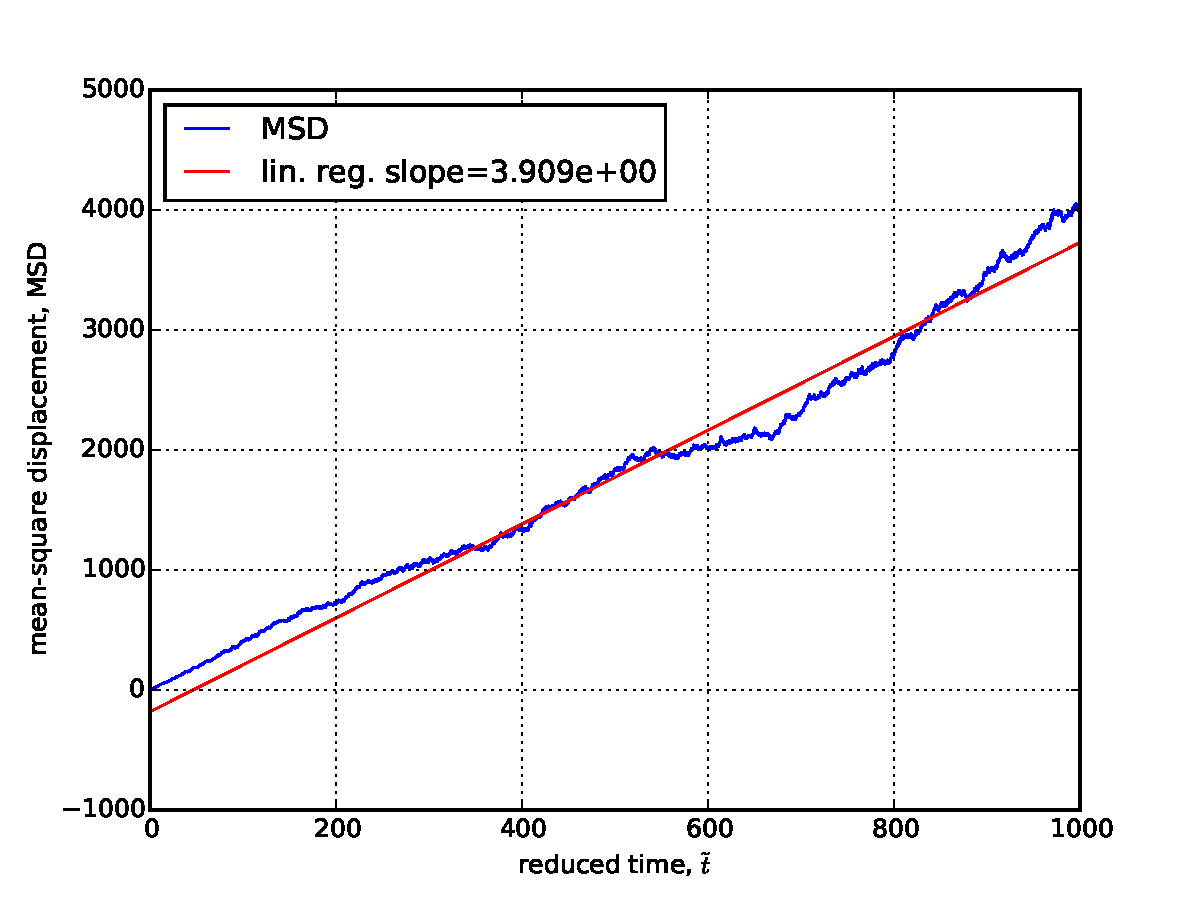
\includegraphics[width=\textwidth]{figures/MSD_2d_Brownian.pdf}
  \caption{MSD for pure Brownian simulation with 1000 reduced time. The blue line represent MSD profile while the red line is linear regression for it. Notice that the slope on here is $3.909$ that is similar to the 4 by theoretical interpretation.}
  \label{fig:MSD_brownian}
\end{figure}


\chapter{Brownian Motion with Repulsive Potential}
\section{Basic Fomular}
Let assumed there existing repulsive potential between particles on Brownian motion with effective radius. For convenience, let $\mathbf{r}_{ij} = \mathbf{r}_j - \mathbf{r}_i$. When distance between two micelles, $\lvert\mathbf{r}_{ij}\rvert$ are lesser than the diameter of single micelle, $R_0$, the repulsive force is defined by
\begin{equation}
\mathbf{F}^{(r)}(\mathbf{r}_i, \mathbf{r}_j) = \mathbf{F}^{(r)}(\mathbf{r}_{ij}) = -C\frac{k_BT}{R_0}\left(1 - \frac{\mathbf{r}_{ij}^2}{R_0^2}\right)\hat{\mathbf{r}}_{ij} \label{eq:force_repulsion}
\end{equation}
where hat denote directional vector, $R_0$ denote expected size for micelle, and non-dimensional parameter $C$ is given by
\begin{equation}
C = \frac{9}{\pi}n_p^2N^{0.2}
\end{equation}
with number of polymer in micelle, $n_p$, and Kuhn number for each polymer, $N$.


From evolution equation of Brownian motion, equation \eqref{eq:evolution_Brownian}, we can add repulsive force to the existing equation as
\begin{equation}
\frac{\partial \mathbf{r}}{\partial t} = \frac{1}{\zeta}\left(\sum \mathbf{F}^{(r)} + \mathbf{F}^{(s)}\right),\label{eq:evolution_Brownian_repulsion}
\end{equation}
where $\mathbf{F}^{(r)}$ is repulsive force and $\mathbf{F}^{(s)}$ is random force contribution. With simple Euler approach, we can represent the given evolution equation as
\begin{equation}
\mathbf{r}(t + \delta t) = \mathbf{r}(t) + \frac{1}{\zeta}\sum\mathbf{F}^{(r)}(t)\delta t + \delta \mathbf{r},\label{eq:update_position}
\end{equation}
where stochastic step, $\delta\mathbf{r}$ is given by equation \eqref{eq:stochastic_step}.

\section{Non-dimensionalization with prefactor C}
Appropriate non-dimensionalization should made order of unity for the reduced (basic) variables. That means, the time scale should be involved the stifness for each potential, i.e., repulsive potential on this article. So, re-defined characteristic time becomes
\begin{equation}
t_c = \frac{\zeta R_0^2}{k_BT}\frac{1}{C},\label{eq:characteristic_time_C}
\end{equation}
while characteristic length is given constant, $R_0$.
Then, we have
\begin{equation}
\tilde{\mathbf{r}}(\tilde{t} + \delta \tilde{t}) = \tilde{\mathbf{r}}(\tilde{t}) + \sum_{i,j}\tilde{\mathbf{F}}^{(r)}(\tilde{\mathbf{r}}_i, \tilde{\mathbf{r}}_j)\delta \tilde{t} + \tilde{\mathbf{F}}^{(s)}\sqrt{\delta\tilde{t}},
\end{equation}
with
\begin{align}
\tilde{\mathbf{F}}^{(r)}(\tilde{\mathbf{r}}_i, \tilde{\mathbf{r}}_j) &= -\left(1-\tilde{\mathbf{r}}_{ij}^2\right)\frac{\tilde{\mathbf{r}}_{ij}}{\tilde{r}_{ij}}\\
\tilde{\mathbf{F}}^{(s)} &= \sqrt{\frac{2}{3}}\tilde{\mathbf{R}}
\end{align}
On this regards, the repulsive potential contribution is following
\begin{equation}
U(\mathbf{r}_i, \mathbf{r}_j) = U(\mathbf{r}_{ij}) = \frac{1}{3}\left(1 + \tilde{\mathbf{r}}_{ij}\right)^2(2 + \tilde{\mathbf{r}}_{ij}).
\end{equation}

It is noteworthy that the repulsive coeffficient, $C$, effect to the system. If it is order of unity, both of repulsive and random forces are comparable. If $C\sim 5900$, the contribution for random force is $\sim 1/77$.

From now on, the dimensionless scheme is following the prefactor one.

\section{Simulation Results}
\subsection{Note}
The basic scheme on here is following the pure Brownian motion. 

\subsection{Trajectory Analysis}

\subsection{Distance and Energy Distribution}
Since the proposed scheme is purely configurational one, the velocity autocorrelation cannot be obtained during simulation. On this regards, the distribution functions for the spatially related one, such as distance between beads, are of importance to study and judge equilibrium conditions. To obtain cumulative distribution function and probability distribution function is described on \label{appen_distance_distribution}.
Figure \ref{fig:CDF_PDF_repulsion} represent the distance distribution for the system with 100 beads and 80 beads with C is equal to the 100 as testing purpose.
The figure showed the slightly different maximum probability distance. One of the main reason for shifted maximum probability distance is that the minimum potential happens even inside effective range because of density of particles. It is clear when we see figure \ref{fig:distance_distribution_repulsion}, which clearly shows the trend.
Since the repulsion is not so stiff, the distance distribution showed relatively broad peaks around 1.0. If we consider the 

\begin{figure}
  \centering
  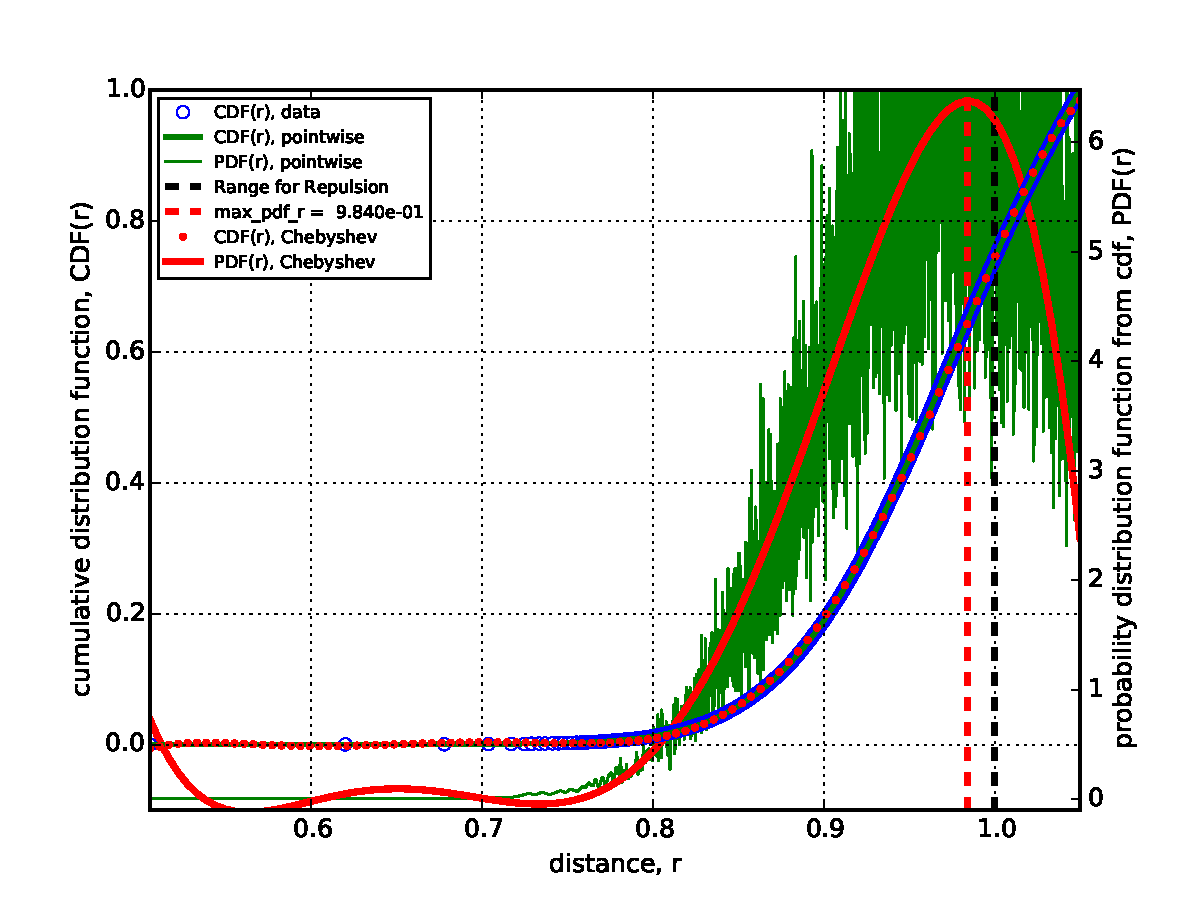
\includegraphics[width=\textwidth]{figures/100_K8.pdf}
  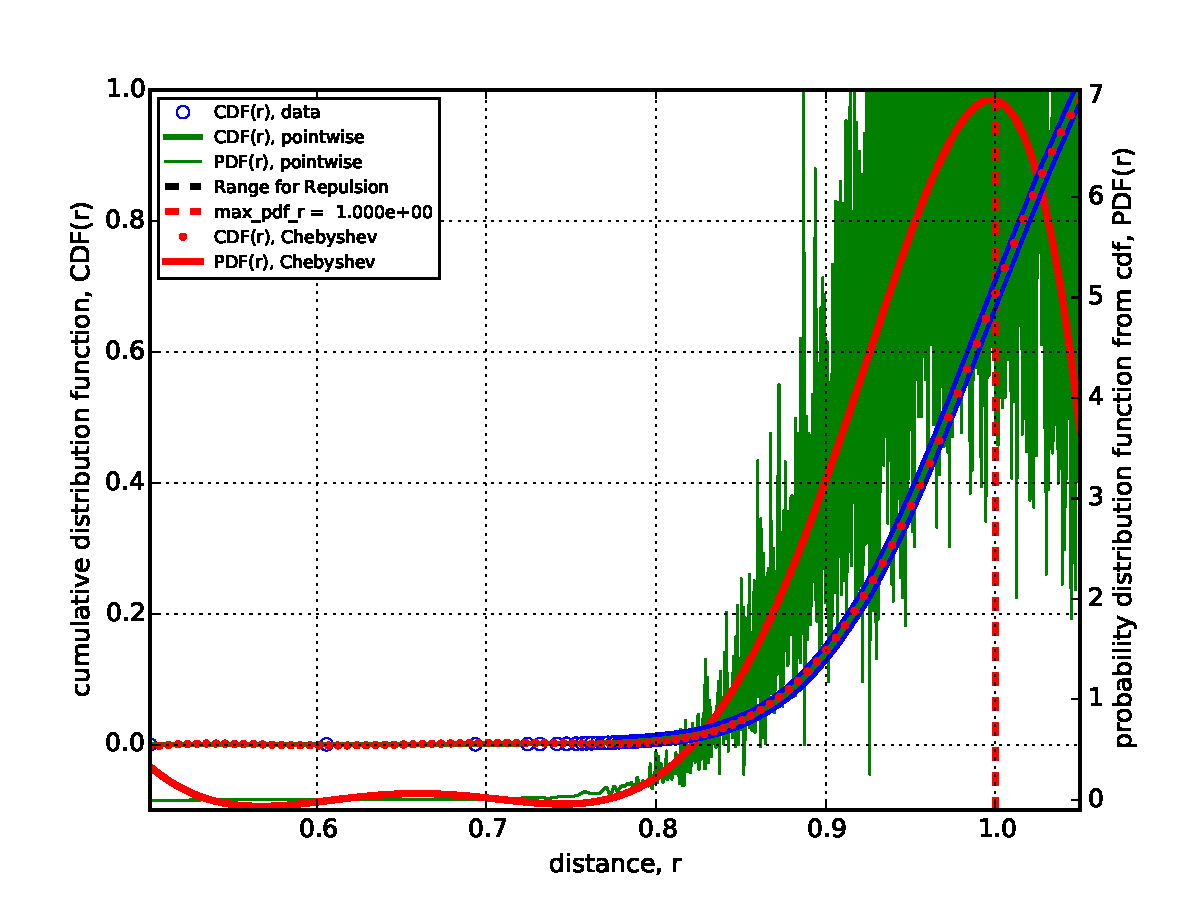
\includegraphics[width=\textwidth]{figures/80_K8.pdf}
  \caption{Cumulative distribution and probability distribution function for NP = 100 (up) and NP = 80 (down). The red color represent the regression, green color represent the interpolation for piece-wise cubic spline, and blue circle represent cumulative distribution from data.}\label{fig:CDF_PDF_repulsion}
\end{figure}

\begin{figure}
  \centering
  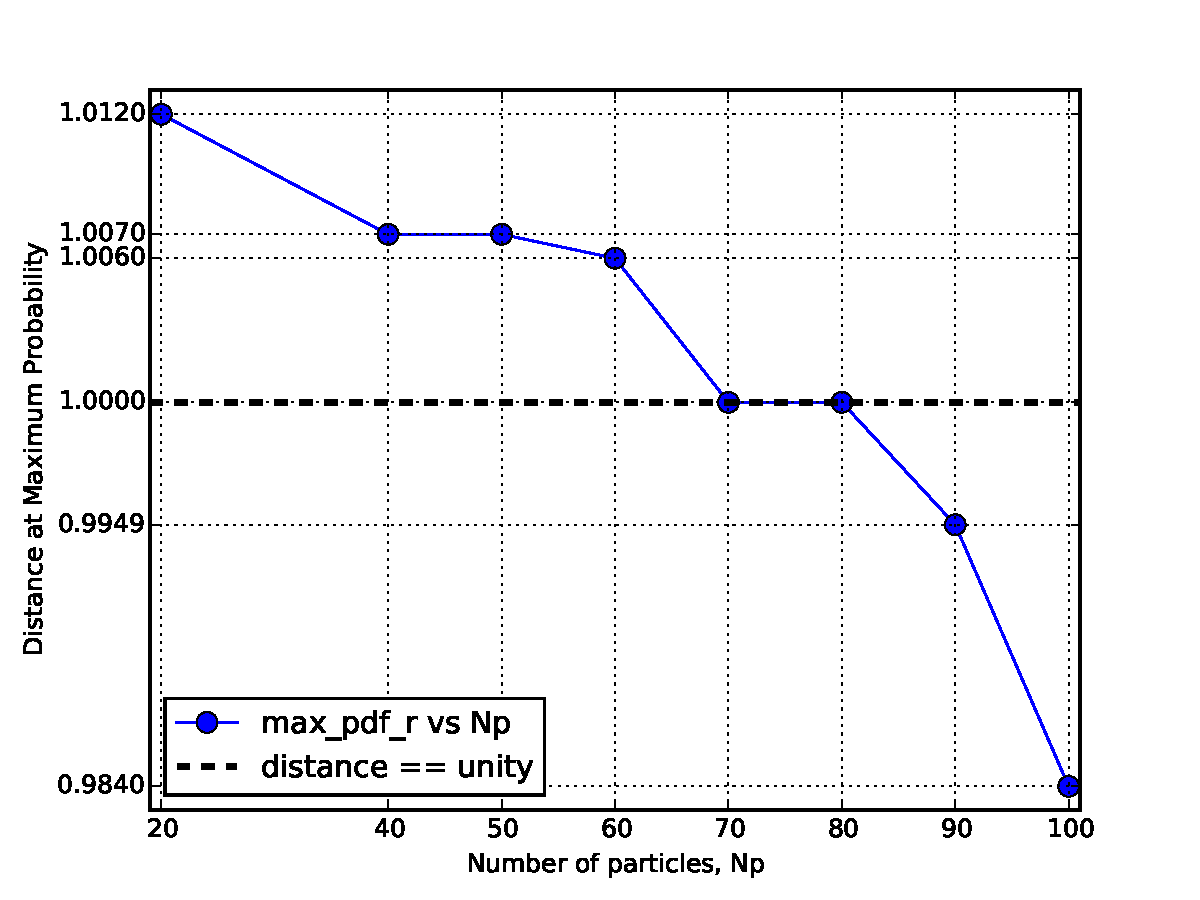
\includegraphics[width=\textwidth]{figures/distance_dist.pdf}
  \caption{Maximum probability distance due to number of particles.}\label{fig:distance_distribution_repulsion}
\end{figure}






\chapter{Brownian Dynamics for Associative System}
\section{Evolution Equations for Associative System}
The evolution equation is simply derived by adding association contribution to the equation \eqref{eq:evolution_Brownian_repulsion}. The results is described on here:
\begin{equation}
\frac{\partial \mathbf{r}}{\partial t} = \frac{1}{\zeta}\left(\sum_{i}\sum_{\substack{j>i,\\j\in\mathscr{C}_i}} \mathbf{F}^{(c)}(\mathbf{r}_i, \mathbf{r}_j) + \sum_i \mathbf{F}^{(r)}_i + \mathbf{F}^{(s)}\right),\label{eq:evolution_Brownian_repulsion_association}
\end{equation}
where $\mathscr{C}_i$ is set of index for the beads associated to the i-th beads and the connected force. 

\subsection{Gaussian Connector}
If we assumed that the connected chain is in Gaussian, we have potential 
\begin{equation}
U^{(c)}(\mathbf{r}_i, \mathbf{r}_j) = U^{(c)}(\mathbf{r}_{ij}) = \frac{N_D}{2}k_BT\frac{\mathbf{r}_{ij}^2}{R_0^2},
\end{equation}
it implies 
\begin{equation}
\mathbf{F}^{(c)}(\mathbf{r}_i, \mathbf{r}_j) = N_Dk_BT\frac{\mathbf{r}_{ij}}{R_0^2}.
\end{equation}
Therefore, the dimensionless potential and force become
\begin{align}
  \tilde{U}^{(c)}(\tilde{\mathbf{r}}_{ij}) &= \frac{N_D}{2}\tilde{\mathbf{r}}_{ij}^2,\\
  \tilde{\mathbf{F}}^{(c)}(\tilde{\mathbf{r}}_{ij}) &= N_D\tilde{\mathbf{r}}_{ij}.
\end{align}

\subsection{Finite Extensible Connector}
The original approach for finite extensible chain is come from \textcite{Kuhn1942}, and the simpler form is derived from \textcite{James1943}. From this results, the potential for finite extensible chain is in complicate form as \parencite{treloar1975physics}
\begin{equation}
U=-k_BTn\left\{\log\left[4\pi\sinh\left(\frac{fb}{k_BT}\right)\right]-\log\left(\frac{fb}{k_BT}\right)\right\},
\end{equation}
where $n$ and $b$ are number and length of Kuhn segment, respectively.
From inverse maps for Langevin function, $\mathscr{L}^{-1}$, the final form for force with finite extensibility becomes
\begin{equation}
  f = \frac{k_BT}{b}\mathscr{L}^{-1}\left(\frac{r}{nb}\right).
\end{equation}
Since there is no closed form of inverse Langevin function, various approximation is derived. \textcite{Cohen1991} derived quite simple but accurate form using Pad\`e approximation:
\begin{equation}
  \mathscr{L}^{-1}(\lambda) = \lambda\frac{3 - \lambda^2}{1-\lambda^2} + O(\lambda^6).
\end{equation}
Note that the $3$ in the formula is not come from spatial dimension, but it is due to the approximation of inverse Langevin function.

Both of potential and force described on above are in complicate to handle. On this regards,  alternative finite extensible form suggested by \textcite{HaroldR.Warner1972} which is frequently called FENE (Finite Extendable Nonlinear Elastic) connector:
\begin{equation}
  f = \frac{k_BT}{b}\frac{3\frac{r}{nb}}{1-(r/nb)^2}.
\end{equation}
Here, prefactor $3$ is regarded as spatial dimension in comparison with Gaussian spring. 
From FENE connector, using we can derive potential by integrating over vector, $\mathbf{r}$.
Using the maximally extendable length, $R_M$, and the mean-square equilibrium end-to-end distance, $R_0$, the potential and force becomes
\begin{align}
U(\mathbf{r}) &= - \frac{N_D}{2}k_BT\left(\frac{R_M}{R_0}\right)^2\log\left(1 - \frac{\mathbf{r}^2}{R_M^2}\right) \\
\mathbf{F}(\mathbf{r}) &= k_BT\frac{R_M}{R_0^2}\frac{N_D\frac{\mathbf{r}}{R_M}}{1-\frac{\mathbf{r}^2}{R_M^2}}.
\end{align}
In comparison with Gaussian spring, the force becomes
\begin{equation}F_
\mathbf{F}(\mathbf{r}) = F_N\mathbf{F}_G(\mathbf{r}),
\end{equation}
where $\mathbf{F}_G$ is Gaussian spring and the non-Gaussian factor $F_N$ is given by
\begin{equation}
F_N = \frac{1}{1-\frac{\mathbf{r}^2}{R_M^2}}.\label{eq:non_Gaussian_factor}
\end{equation}
The non-dimensionalized form becomes
% Using $R_0=\sqrt{n}b(=1)$ as characteristic length, we can non-dimensionalization as
\begin{align}
\tilde{U}(\tilde{\mathbf{r}}) &= -\frac{N_D}{2}\left(\frac{R_M}{R_0}\right)^2\log\left(1-\frac{\tilde{\mathbf{r}}^2}{(R_M/R_0)^2}\right),\\
\tilde{\mathbf{F}}(\tilde{\mathbf{r}}) &= \left(\frac{1}{1 - \frac{\mathbf{r}^2}{(R_M/R_0)^2}}\right)\tilde{\mathbf{F}}_G(\tilde{\mathbf{r}}) \equiv \tilde{F}_N\tilde{\mathbf{F}}_G(\tilde{\mathbf{r}}).
\end{align}
Notice that the non-Gaussian factor $\tilde{F}_N$ is the same with \eqref{eq:non_Gaussian_factor}:
\begin{equation}
\tilde{F}_N = \frac{1}{1 - \frac{\mathbf{r}^2}{(R_M/R_0)^2}} = F_N.
\end{equation}

As reference point of view, \textcite{Ianniruberto:2015dv} use $R_M/R_0 = 11$ which this will add for the code as additional parameter.
% In comparison with Gaussian spring, we can use the form
% \begin{equation}
% \tilde{\mathbf{F}}(\tilde{\mathbf{r}}) = \tilde{F}_N\tilde{\mathbf{F}}_{G}(\tilde{\mathbf{r}})
% \end{equation}
% with
% \begin{equation}
% \tilde{F}_N
% \end{equation}
% \begin{align}
% \tilde{U}(\tilde{\mathbf{r}}) &= -\frac{N_D}{2}\left(\frac{R_M}{R_0}\right)^2\log\left(1 - \frac{\tilde{\mathbf{r}}^2}{(R_M/R_0)^2}\right) = -frac{N_D}{2},\\
% \tilde{\mathbf{f}}(\mathbf{r}) &= 
% \end{align}


% The detail potential for the original finite extensibility is come by complicate form. From assumption of constant force exerted on each end of chain, $\mathbf{f}$, the potential energy, $u$, can be expressed in terms of the constant force and end-to-end vector, $\mathbf{R}$, as follow:
% \begin{equation}
% u = -\int_0^R\mathbf{f}\cdot d\mathbf{r} = -\mathbf{f}\cdot\mathbf{R} = -fh_z,
% \end{equation}
% where $h_z$ is sum over all the projection of segmental vector to the $\hat{\mathbf{R}}$. Then we have $T-f-N$ partition function:
% \begin{equation}
% Z(T, f, N)=\sum_{state}\exp\left(\frac{fh_z}{k_BT}\right)\approx\left[4\pi\frac{k_BT}{fh_z}\sinh\left(\frac{fh_z}{k_BT}\right)\right]^N.
% \end{equation}
% Then we have potential as
% \begin{align}
% U &= -k_BT\log Z(T, f, N) \\
% &=-k_BTN\left\{\log\left[4\pi\sinh\left(\frac{fb}{k_BT}\right)\right]-\log\left(\frac{fb}{k_BT}\right)\right\},
% \end{align}
% where $b$ and $N$ are length and number of Kuhn segment, respectively. From here, we have
% \begin{equation}
% \langle R\rangle = -\frac{\partial U}{\partial f} = bN\mathscr{L}\left(\frac{fb}{k_BT}\right),
% \end{equation}
% where $\mathscr{L}$ denotes Langevin function given by
% \begin{equation}
% \mathscr{L}(x) = \coth(x)-\frac{1}{x}.
% \end{equation}

\section{Implementation for Association}
%% Basic assumptions:
%% \begin{enumerate}
%% \item The association is determined before solving evolution equation
%% \item Determination for the association is using Monte Carlo simulation with transition state
%% \item Each Monte Carlo trial, the beads for visiting is randomly choosen
%% \item Each visited beads is assumed that transition state, and 
%% \end{enumerate}

%% \section{Probability}
First of all, the association is pre-determined before solving evolution equation. The expected algorithm is described on below.
\begin{enumerate}
\item Visiting randomly selected bead
\item Selecting chains on the bead as transition state based on the $Z_k$
\item Determine the behaviour of specific chains based on Gaussian distribution
\item Loop until the potential energy is in equilibrium
\end{enumerate}
These steps does not vary the time, instant time, and determine the association information for evolution equation. When initial box is generated, the position is equilibrated without applying association. Then the core of simulation is experience the loop of association step (instant time) up to equilibrium based on number of association and solving evolution equation for next time step. At this moment, each association step does not inherit, which means the information for bridges are re-set when new instant time is given. This is due to testing purpose since the state variables should invariance from history of selection. However, from this option, the computing time for association step occupy more than 99{\%} of all computing expenses, which will be dramatically reduced when switch off the renewal bridge options.

\subsection{Equilibration for Each Association Step}
It is of importance to judge the equilibrium due to MC steps for time optimization. The simple way is using number of associations as state variables, then the equilibrium identify is based on this value. Here, I have used number of association averaged over previous times, then taking numerical differentiation. The block average for numerical differentiation is applied. Let $N_b(m)$ be number of bridge chains at step $m$. The averaged over previous time in discretized form is given by
\begin{equation}
\bar{N}_b(m_K) = \frac{1}{K}\sum_{k=1}^{K}N_b(m_k).
\end{equation}
Then, the difference of evolving time is given by
\begin{align}
\bar{N}_b(m_{K}) - \bar{N}_b(m_{K-1}) &= \frac{1}{K}\sum_{k=1}^{K}N_b(m_k) - \frac{1}{K-1}\sum_{k=1}^{K-1}N_b(m_k) \\
&= \frac{1}{K(K-1)}\left[(K-1)\sum_{k=1}^{K}N_b(m_k) - K\sum_{k=1}^{K-1}N_b(m_k)\right] \\
&= \frac{1}{K(K-1)}\left[(K-1)N_b(m_K) - \sum_{k=1}^{K-1}N_b(m_k)\right].
\end{align}
The last form has benefit to computing expenses. Since it is averaged value, the convergence rate is slower than the real value, which is good point for avoiding the pathology. The results for one instant time is described in figure \ref{fig:identification_equilibrium_MC}.

\begin{figure}
  \centering
  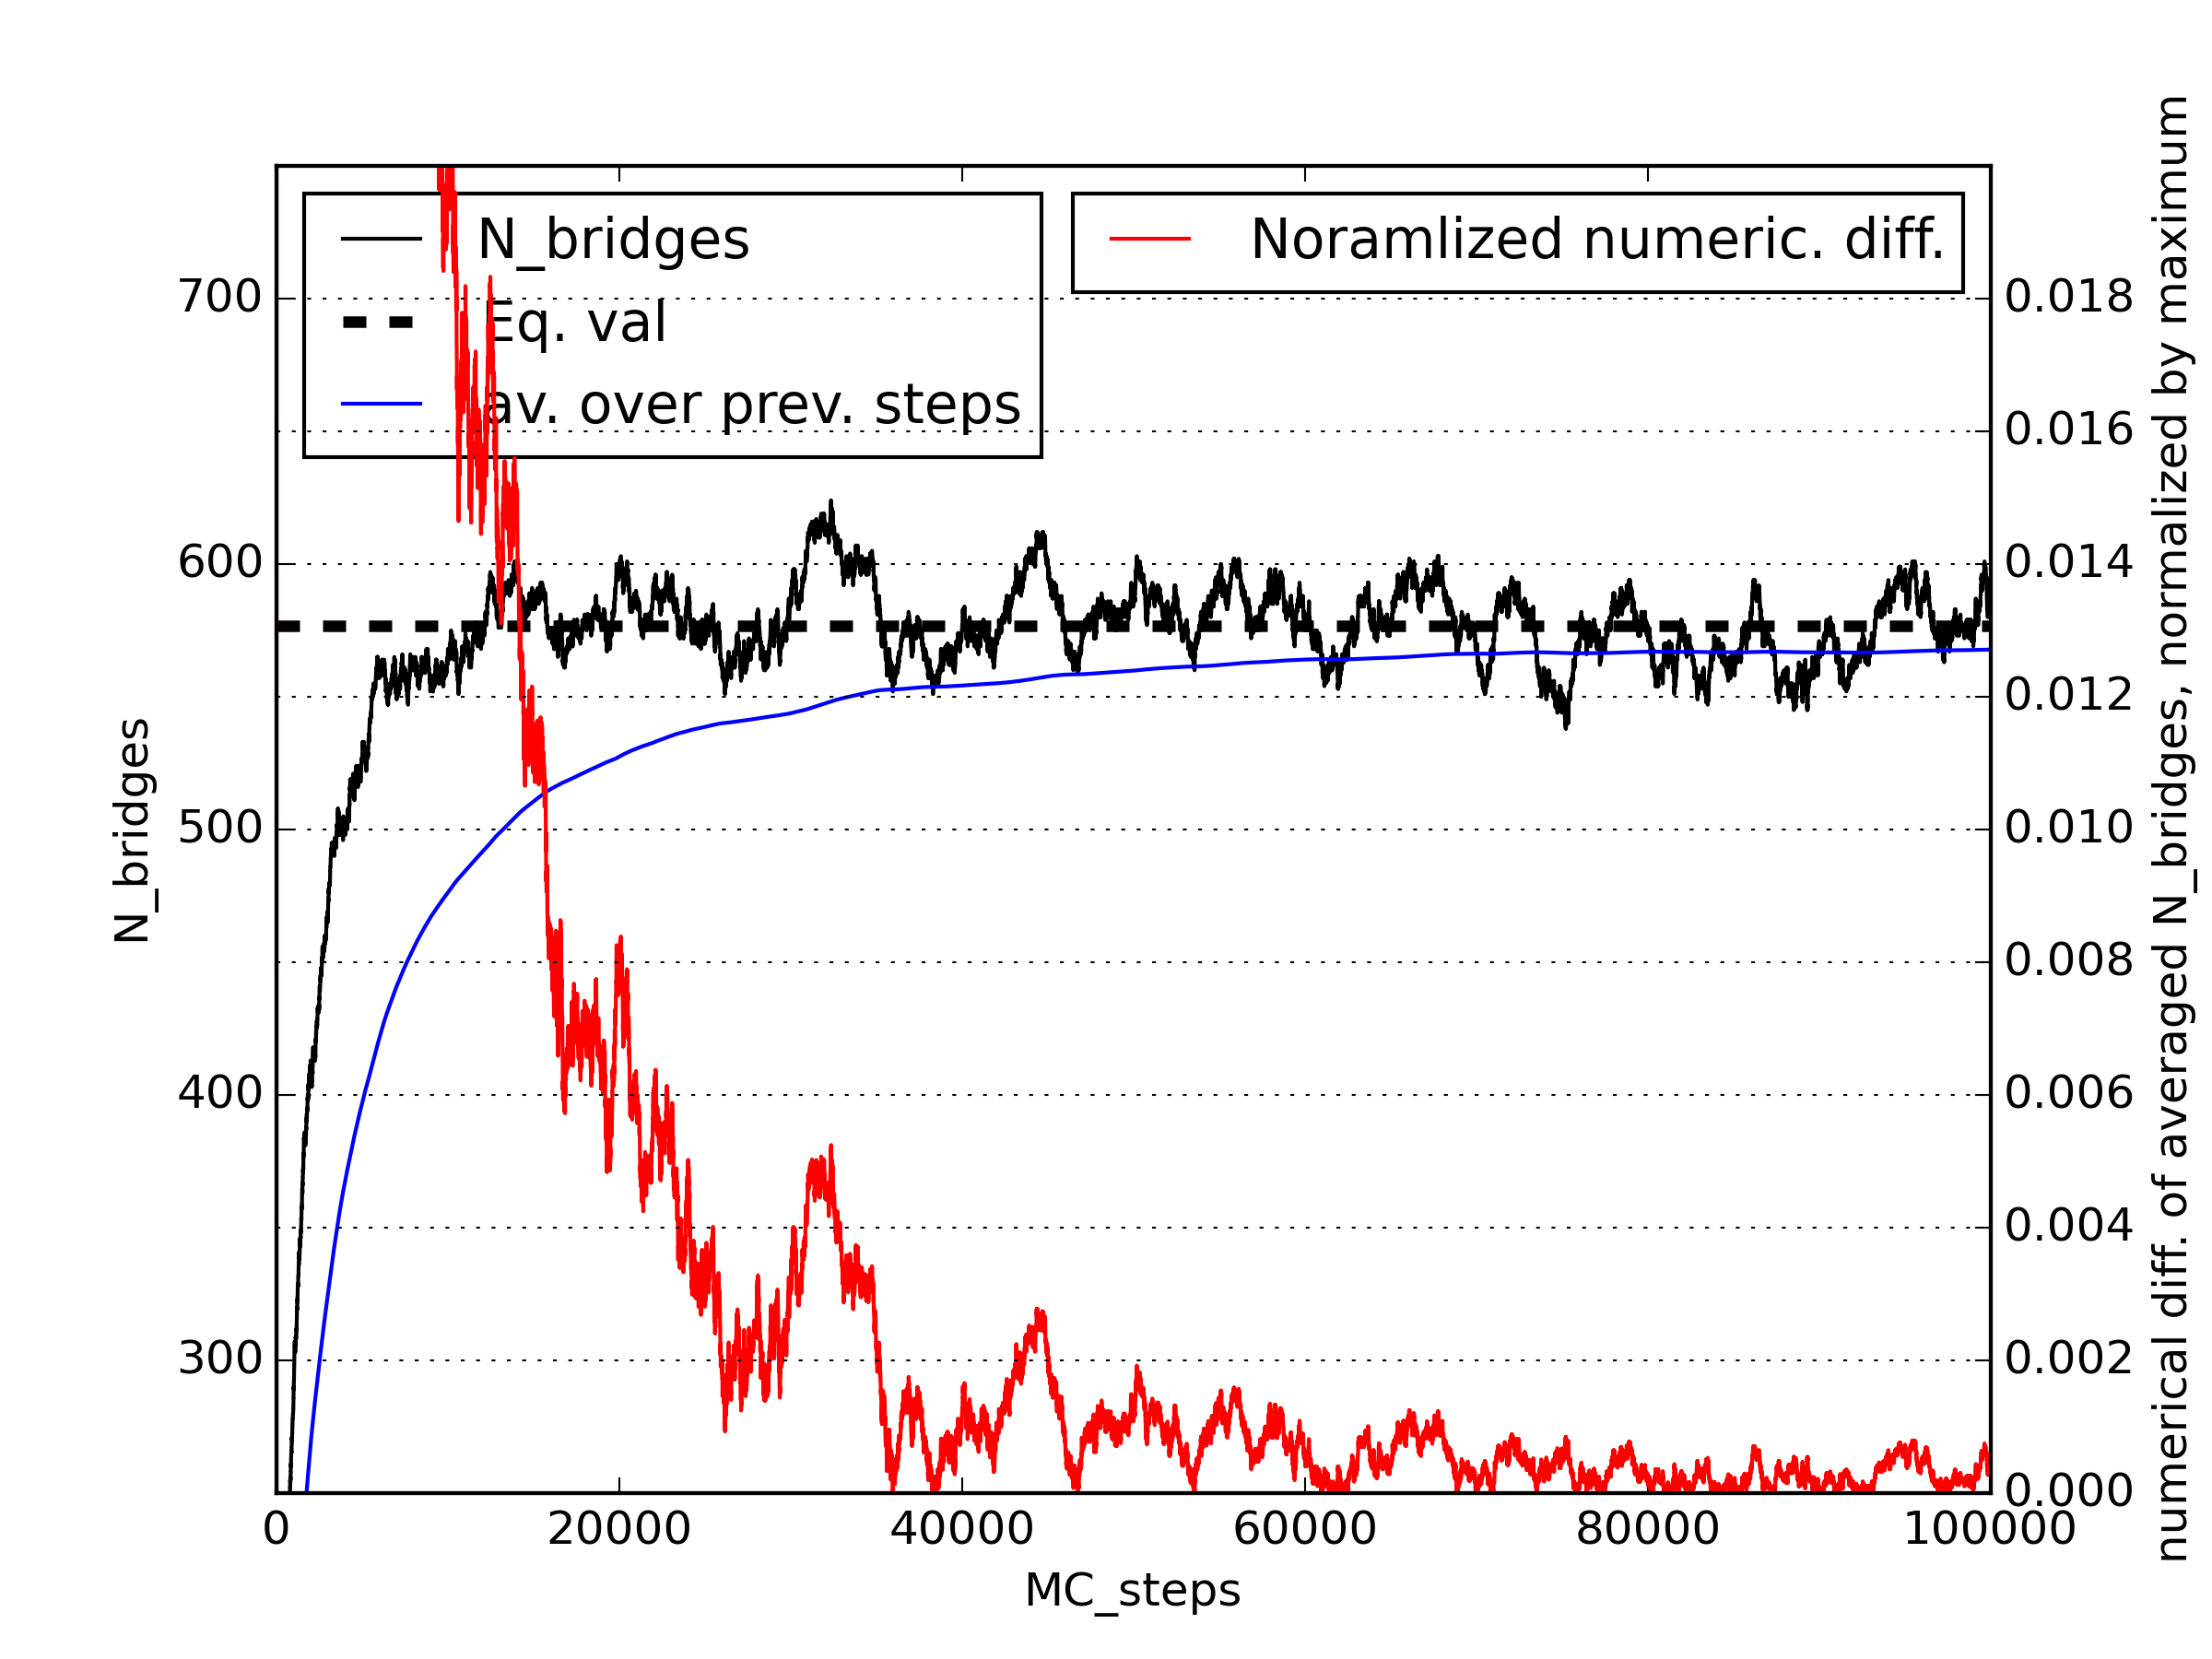
\includegraphics[width=0.8\textwidth]{figures/identify_equilibrium.png}
  \caption{Identification of equilibrium for association steps. The black line represent the number of bridges of each MC step, blue line is the number of bridges averaged over previous time, and the red line is normalized difference value without smoothing. To be safe side, slight smoothing process is applied by using several steps.}
  \label{fig:identification_equilibrium_MC}
\end{figure}

\subsection{Probability to Select Chain in Beads}
Let there $n_p$ chains for each micelle, i.e., the micelle has $2n_p$ of attached chain end. Each chain end allowing to detach from the original micelle and to attach different micelle. Let $U$ be a potential related to the force exerted on the strand between different micelle, we have partition function for a bead, $Z_k$, as follow:
\begin{equation}
  Z_k = \sum_{i=1}^{2n_p}\exp\left(\beta U(\mathbf{r}_i, \mathbf{r}_{\mathscr{C}_k(i)})\right),
\end{equation}
where $\beta = (k_BT)^{-1}$ and $\mathscr{C}_k(i)$ is index for bead that attached i-th chains on k-th beads. Notice that typical Boltzmann factor for partition function is given by $\exp(-\beta H)$ where Hamiltonian is given by $H = T - V$. Therefore, the sign on here is plus.
The given number of case directly suggest that the probability for choosing the chain that will act. For instance, let consider the first beads, $Z_1$, if the beads does not associate with any other bead, the $\mathscr{C}_1(i)$ becomes 1 for all $i\in[1, n_p]$.
From given potential, equation \eqref{eq:Gaussian_potential}, all the potential on each chains become zeros that means the each contribution to the partition function is unity. Therefore, $Z_1$ in this case becomes $2n_p$.

\subsection{Behaviour of Selected Chain}
It is of importance to determine the next step after selection of chain. For given number of beads, $N_B$, the target to attachment is based on the following distance probability:
\begin{equation}
  p_k(\{\mathbf{r}\}\equiv \exp\left(-\beta U(\{\mathbf{r}\} - \mathbf{r}_k)\right),
\end{equation}
where $U$ is given potential and $\{\mathbf{r}\} = \{\mathbf{r}_0, \mathbf{r}_1, \cdots, \mathbf{r}_{N_B}\}$.
% The simple suggestion for the probability can be defined as Gaussian, i.e., $p(r)\sim \exp(-\alpha r^2)$. For given number of beads, $N_B$, the target to attachment is based on the following distance probability:
% \begin{equation}
%   p_k(\{\mathbf{r}\}) \equiv \exp\left(-\beta U(\{\mathbf{r}\}-\mathbf{r}_k)\right) = \exp\left(-\frac{1}{2}N_D\left(\{\mathbf{r}\}-\mathbf{r}_k\right)^2\right), \label{eq:Gaussian_probability}
% \end{equation}
% where $\{\mathbf{r}\} = \{\mathbf{r}_0, \mathbf{r}_1, \cdots, \mathbf{r}_{N_B}\}$.
In addition, it should following the ceiling probability rather than floor one. 
Figure \ref{fig:probability_80} is one example to compute probability from distance distribution. When we roll the random generation from 0 to 1, we make decision where to attach and most probably the original bead.
When we toggle the random number from 0 to 1, the randomly generated number determine newly selected beads. For instance, if the number is 0.4 in figure \ref{fig:probability_80}, then the selected chain will attach for the 0-th bead. Notice that the position of beads are fixed during association steps, the maps for adjacent beads is only computed once to reduce computing price. 
\begin{figure}
  \centering
  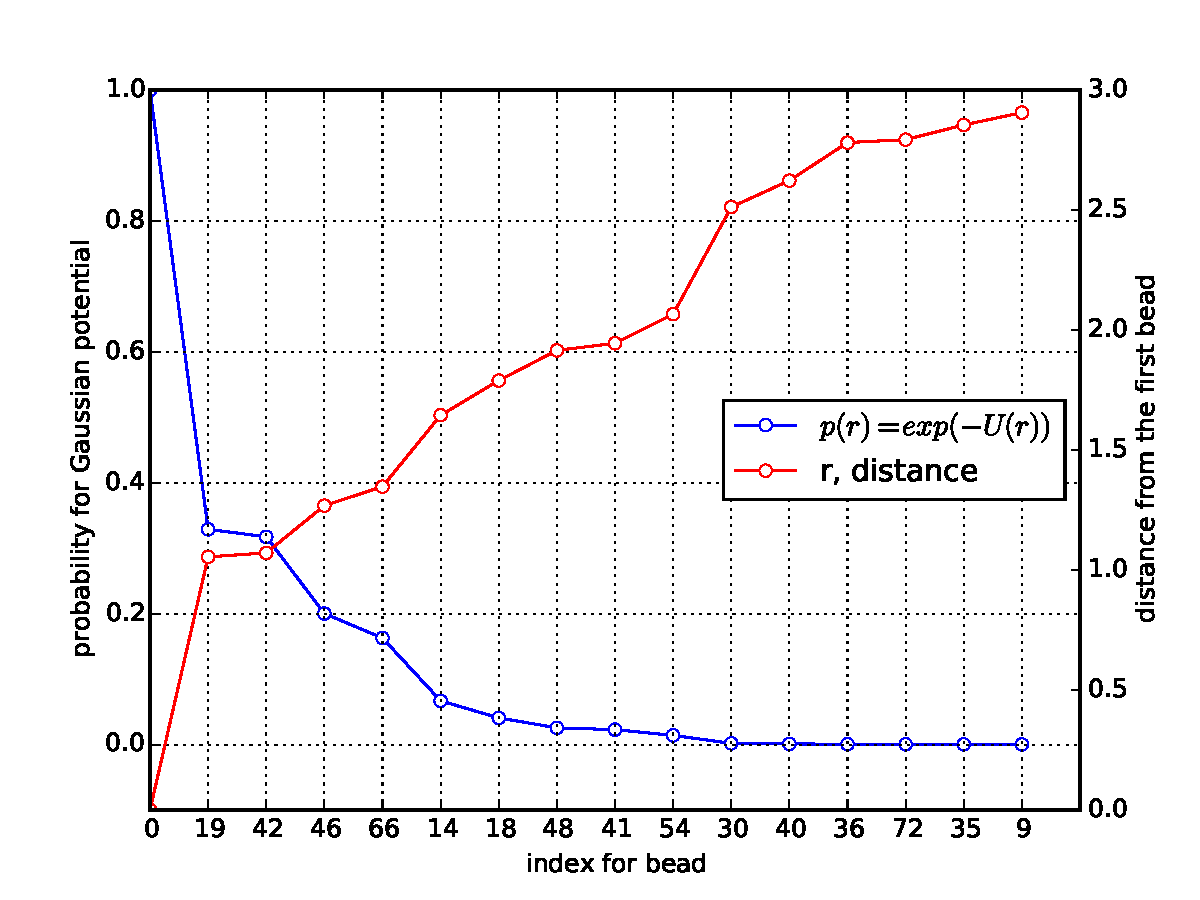
\includegraphics[width=0.8\textwidth]{figures/80_potential_dist.pdf}
  \caption{Example for the probability of chain extension using Gaussian connector. The data is sampling from 80 beads system and only account for repulsive potential (no association). The variables are dimensionless. The red color represent distance from the first bead (index is 0), and the blue color represent probability using Boltzmann factor. }\label{fig:probability_80}
\end{figure}

% \subsection{Restricted Number of Connections}
% It is of importance that the number of connections for one micelle is restricted by 10\% of $2n_p$. For instance, if there is 10 chains on the micelle, we have 20 chain ends. The chain ends attached that micelle is only valid between 18 to 22, which controls the functionality to connect that beads. In any case, if the probability is disagree the given condition, such as maximum or minimum number of connections, the trial is drop and re-rolling is involved like Metropolis algorithm.

\subsection{Allowance for Number of Chain Ends per Bead}
If the number of chain ends attached a beads is constant, the movement of association is the only possible way during Monte-Carlo steps. Hence, it would be importance to check the effects of number of allowance for attached chain ends per bead. Figure \ref{fig:TN_effect} is tested with the 25 chains per bead (i.e., 50 chain ends per bead) and allowing 3, 5, and 7 for the allowance number of fluctuating. It seems to be there is small trend exist due to the allowance number, but in minor. Even if it is quite early to say the total number of association is free from the number of allowance (if it is larger than 3), this will not be major effects for our future works. The results will be re-visited when our algorithms and methods are stable and re-producible.

\begin{figure}
  \centering
  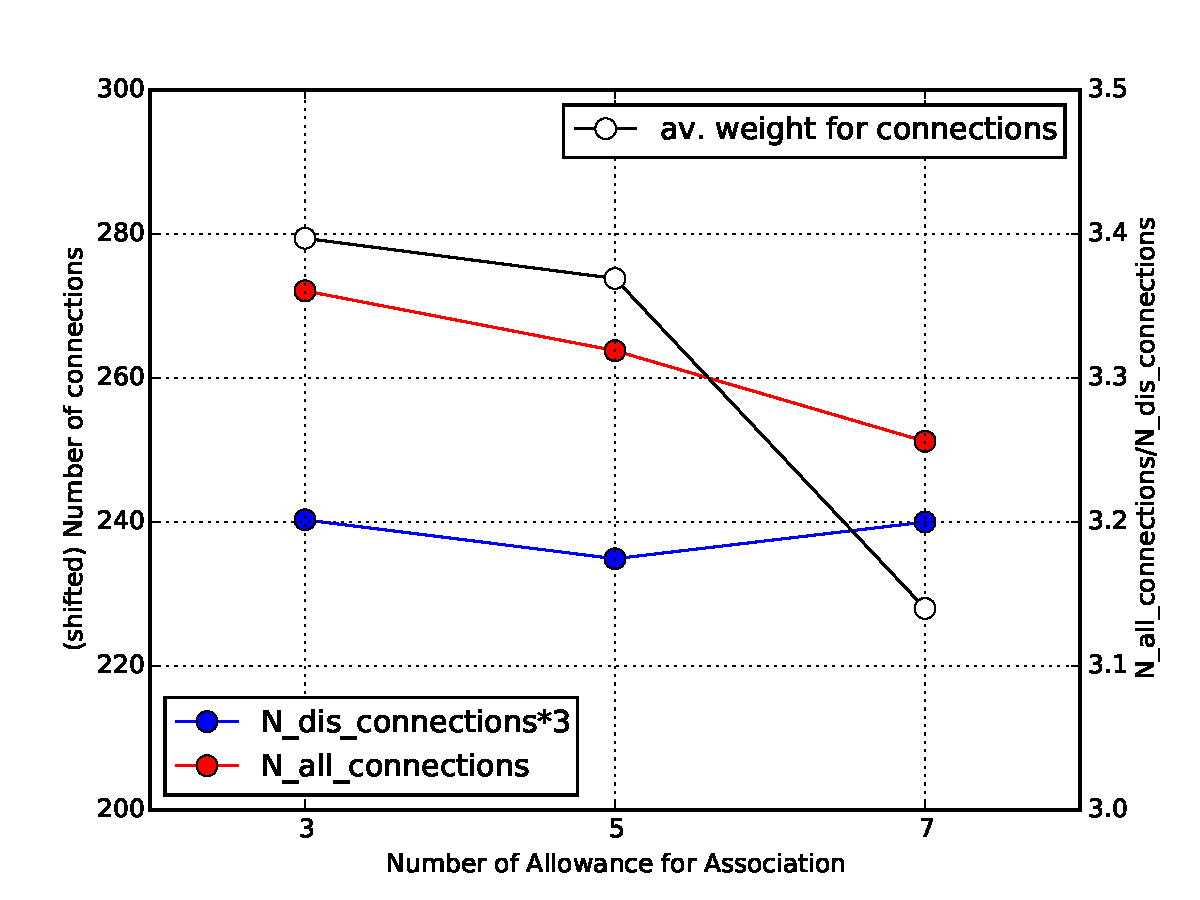
\includegraphics[width=0.8\textwidth]{figures/TN_effect.pdf}
  \caption{Effects of number of allowance for fluctuating attached chain ends per bead. N{\_}dis{\_}connections state number of distinguashable connections, i.e., all different pairs of association, and N{\_}all{\_}connections means number of all bridge chains. The right axis is the ratio between this two counted numbers, which refer intensity per bridge chains.}
  \label{fig:TN_effect}
\end{figure}




\section{Simulation Results}
\subsection{Clustering}
The critical concentration for 100 area box ($10^2$) in dimensionless is based on the figure \ref{fig:distance_distribution_repulsion} that suggest the 80 beads/100 area can be overlap concentration with applied repulsive potential. To be safe side, the 40 beads is selected for testing purpose. Evolving time make clster in the system, which is shown in figure \ref{fig:clustering}. The size effects has been checked that is also reported in figure \ref{fig:clustering}. From this aspect, the given parameter sets may show aggregations. Note that, however, the connecting vector shows isotropic; therefore, the clustering in equilibrium simulation does not deviate from isotropic solution concepts. 

\begin{figure}
  \centering
  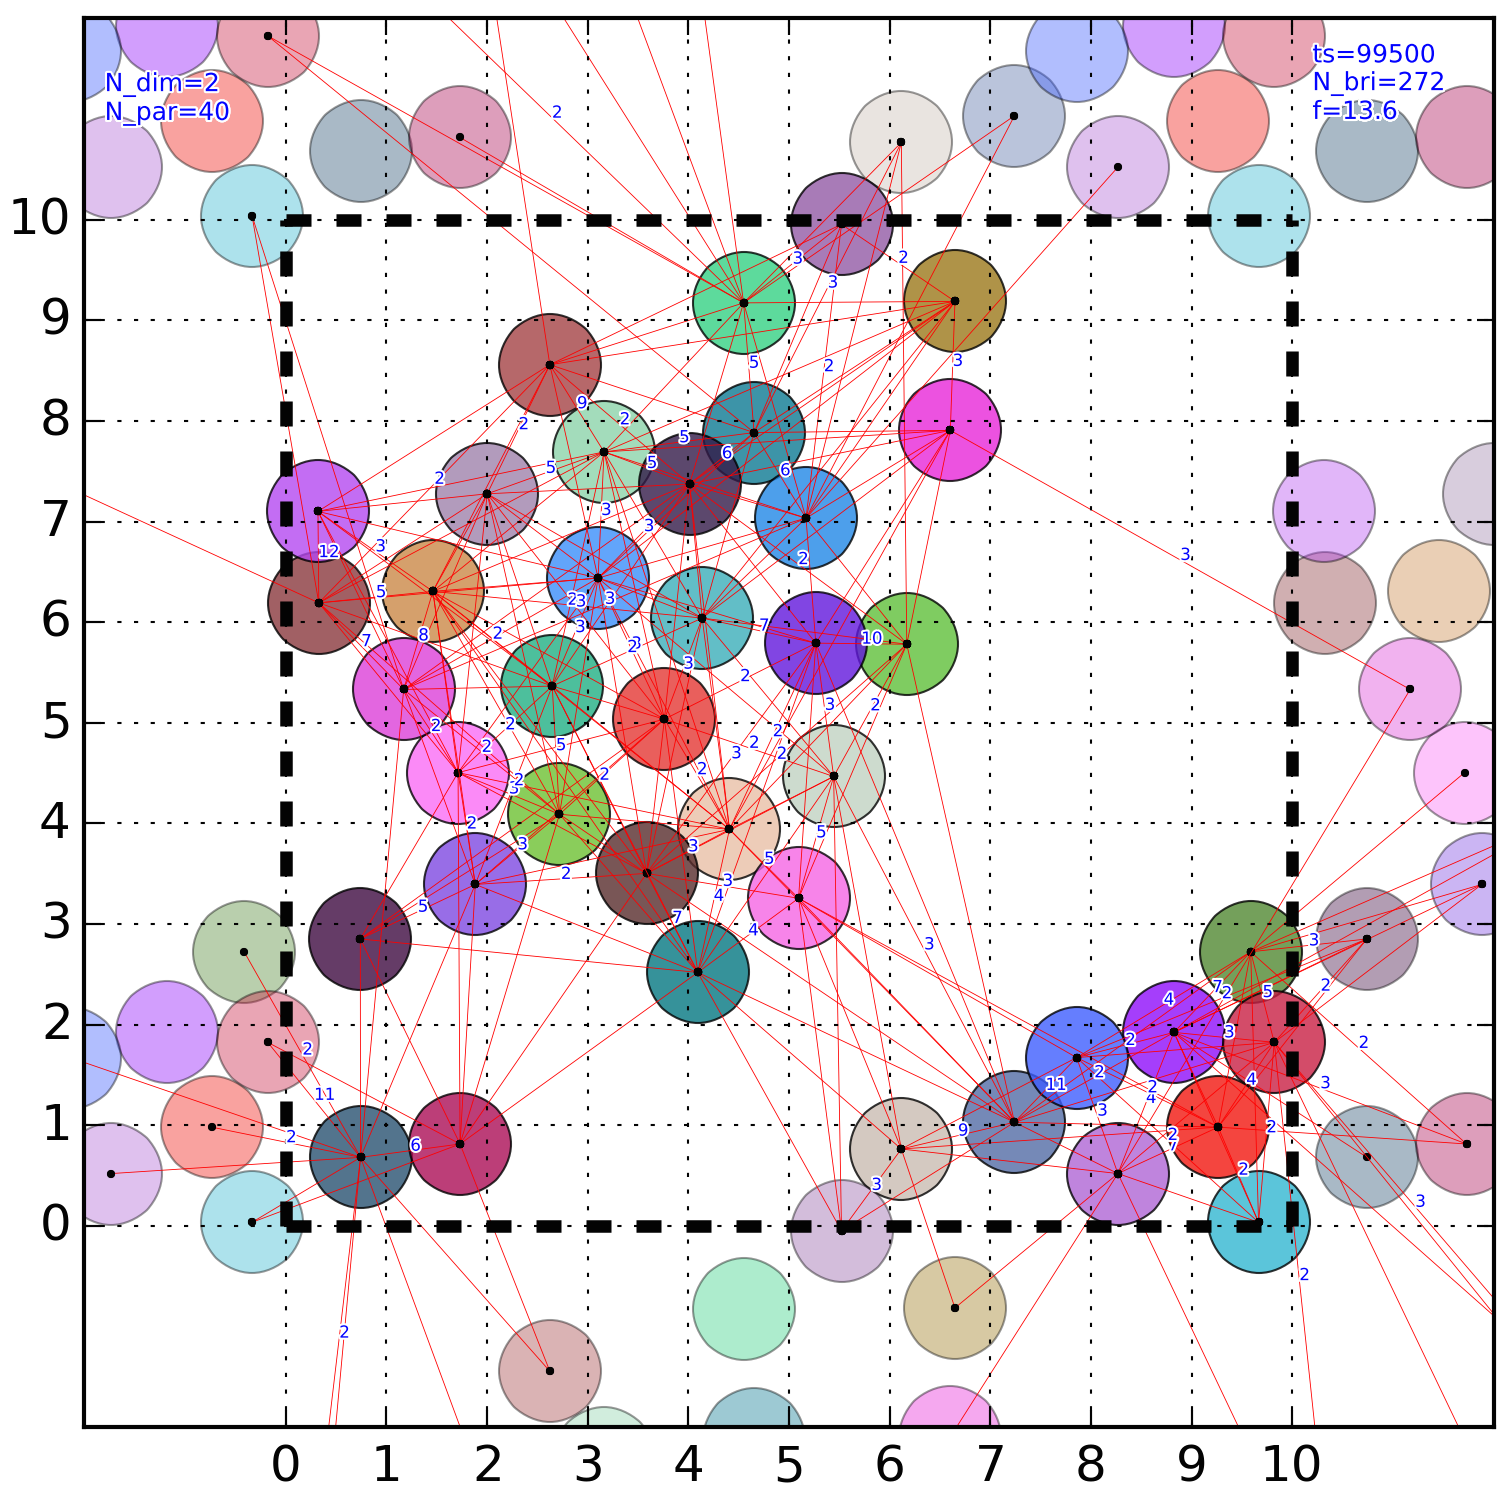
\includegraphics[width=0.49\textwidth]{figures/NP40_A100_clustering.png}
  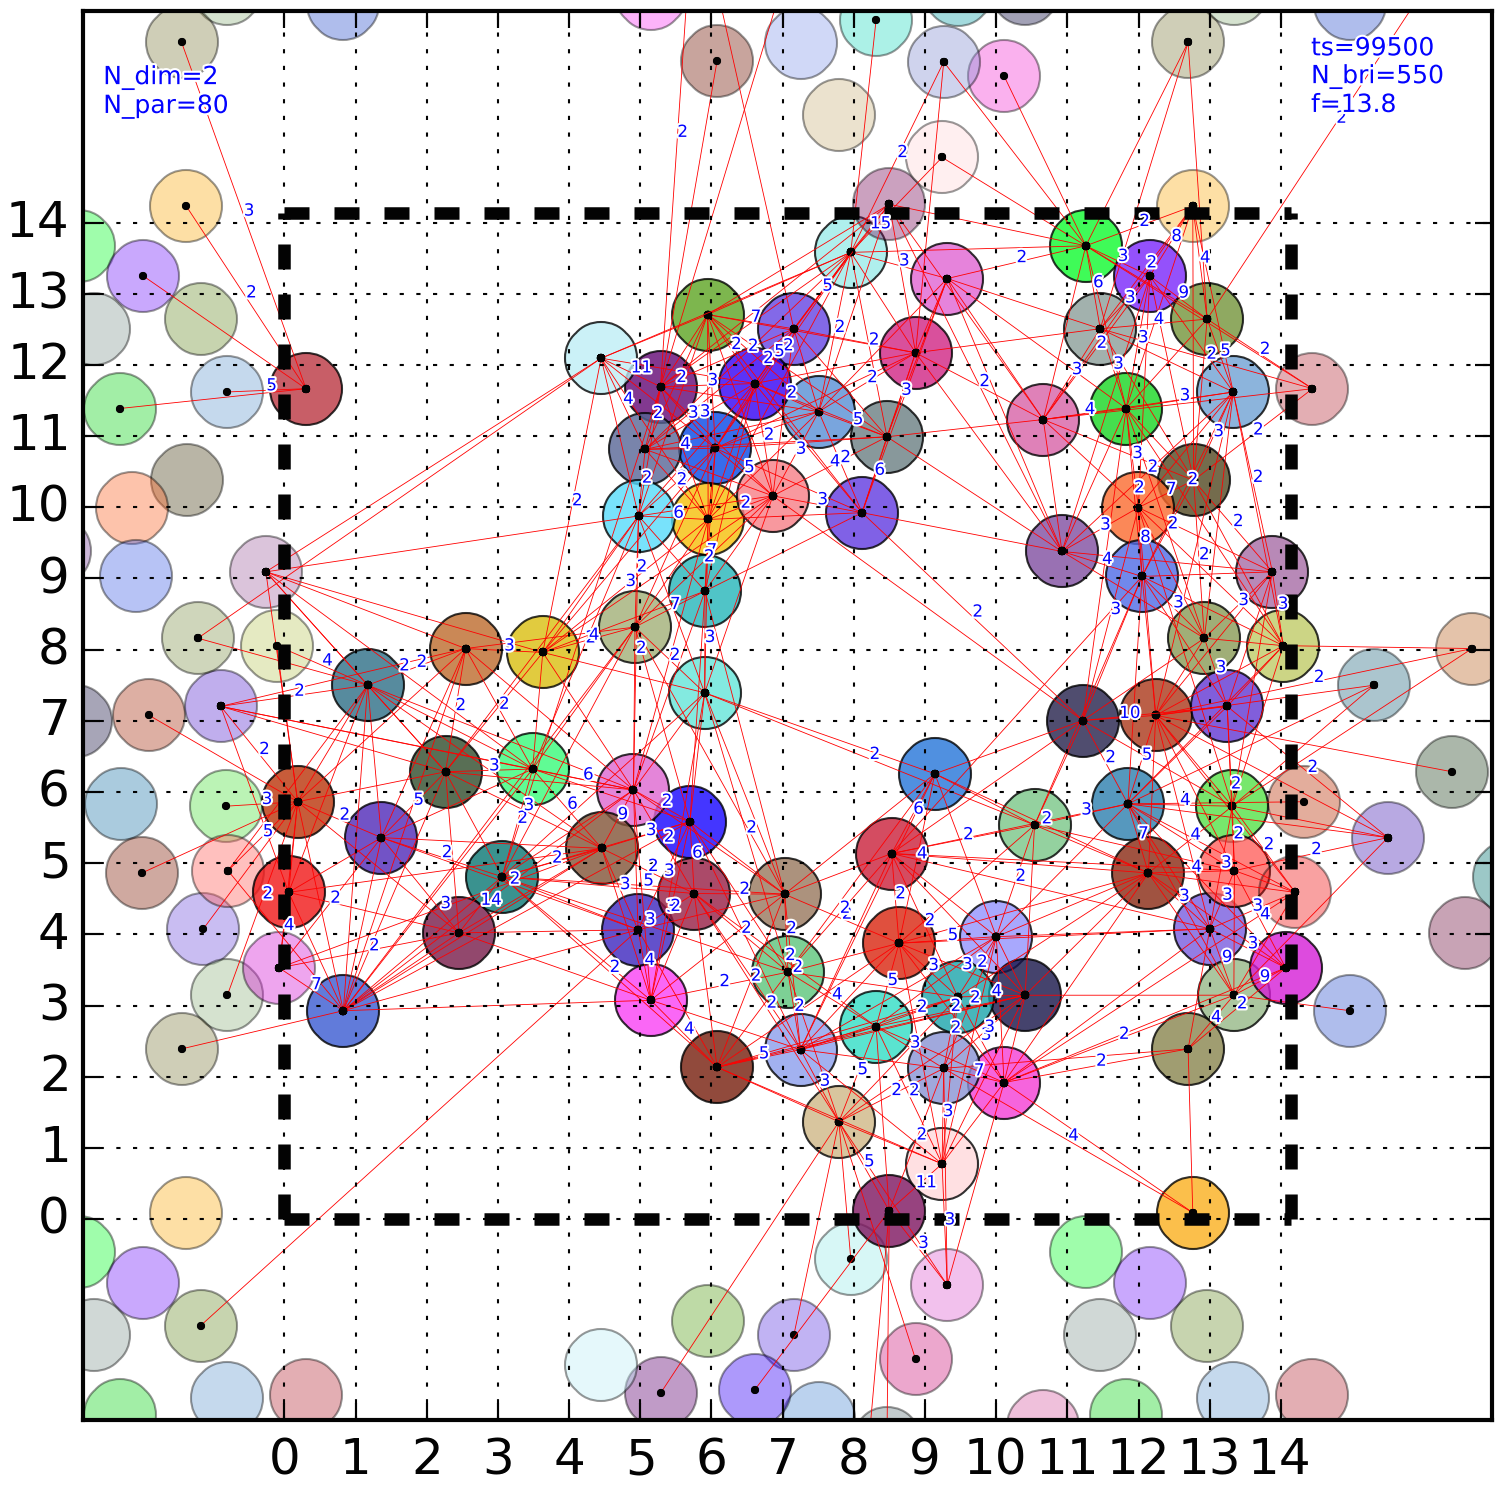
\includegraphics[width=0.49\textwidth]{figures/NP80_A200_clustering.png}
  \caption{Builded cluster during simulation. Both system has the same concentration but different box size.}
  \label{fig:clustering}
\end{figure}



% \subsection{FENE effects}
% Up to now, only Gaussian spring is applied for the association. This results in quite long-range association with quite high probability. It is quite early to analysis effect of finite extensibility. But, it should be check near future.

\subsection{Isotropic for connecting vector}
According to the \textcite{Ianniruberto:2015dv}, the stress tensor is given by
\begin{equation}
\boldsymbol{\sigma} = 3\nu k_BT\bar{f}\langle\mathbf{\tilde{R}\tilde{R}}\rangle,
\end{equation}
where $\nu$ is excluded volume of a monomer of polymer chain, and $\bar{f}$ is non-Gaussian factor which is unity when we use Gaussian spring for association. On this regards, the associative contribution for the stress tensor proportional to the diadic of connecting vector, $\langle\mathbf{RR} \rangle$. On this regards, the isotropy of connecting vector is of importance for equilibrium simulation, which is reported in figure \ref{fig:RR_isotropy}. The initial transition parts (up to 200 time steps) is results of clustering. Notice that the given stress tensor is the only associative part. Hence, the check for the istorpic should be checked with the stress contribution from the repulsive parts and Brownian motion as well.

\begin{figure}
  \centering
  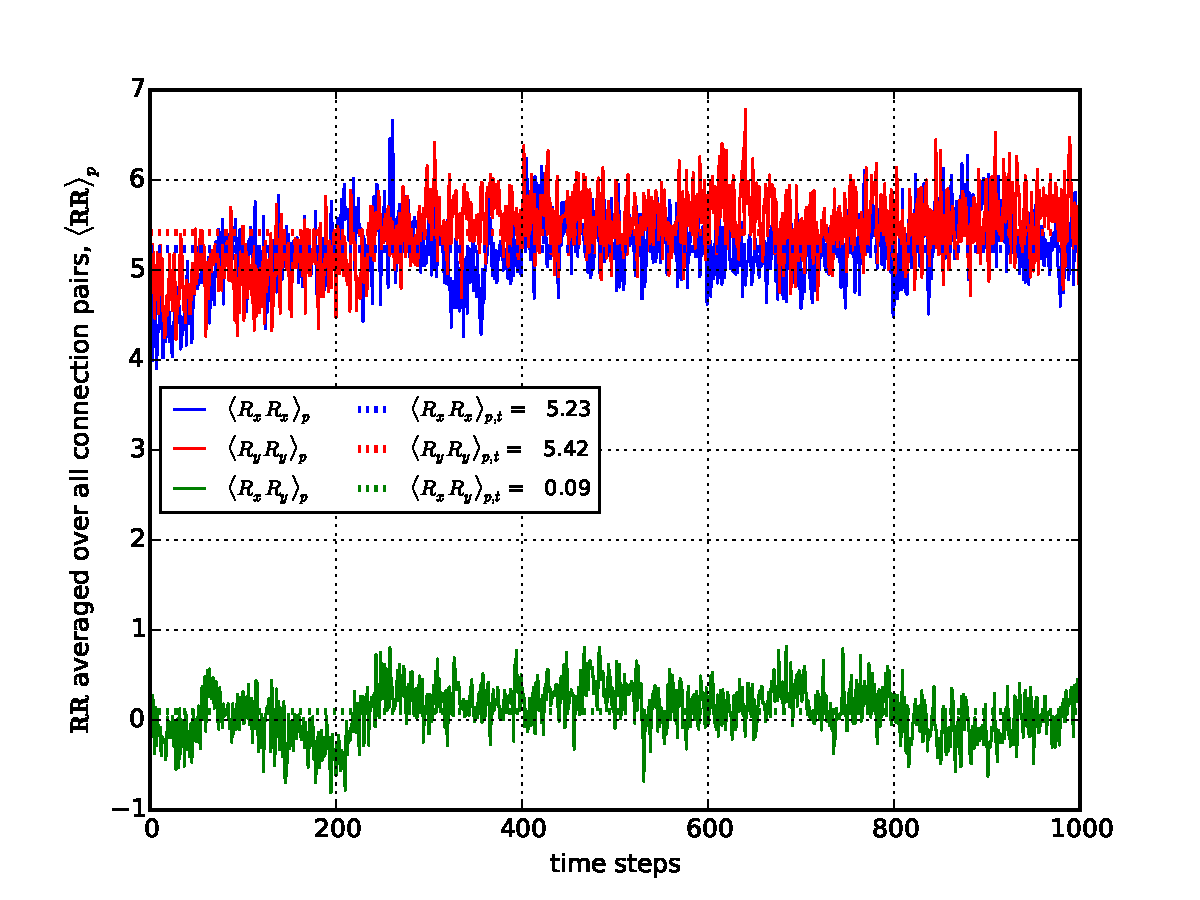
\includegraphics[width=\textwidth]{figures/RR_NP80_C100_T3.pdf}
  \caption{Measured $\langle \mathbf{RR}\rangle_p$ for 80 beads per 200 area system. The diagonal components are almost identical while the off-diagonal components are negligible, which is the sign for isotropy.}
  \label{fig:RR_isotropy}
\end{figure}

\subsection{Size Effects}
The system size is of important factor for dynamics of the system. By doubling system size, we can checked the given system is in experience for the size effects. The simple result is reported in figure \ref{fig:clustering}. \textbf{The other aspects will be checked later on}.

%% \subsection{Some notes for the selection}
%% Note that when the bead is associate, that is one chain end is detached from the original bead and attached to the adjacent bead. It has lower probability. That means, the probability to select the associated chain is reduced while the probability to back to the original beads is increasing. This might be problematic for reducing probability to select, and potentially postpone the time to reach equilibrium condition.


%% \part{Appendix}
\begin{appendices}

  \chapter{Finite Extensibility}
  Describe.

  \chapter{Time Correlated Data}
  \section{Stationary State Variable}
  Let $\mathscr{A}$ be a state variable and the system is in equilibrium. That means the $\mathscr{A}$ is fluctuation around a certain average value $A = \langle \mathscr{A}\rangle_t$ when the system is assumed Ergodic. If the sampling time is sufficiently large, the number for time sampling does not affect to the average value, A. In the case of variance, however, it affected by sampling number since we cannot avoid time correlation between two time steps. It is noteworthy that the average value itself said the first moment of $\mathscr{A}$ while the variance is the second moment. On this regards, we can say the time correlation does affect to the moment of $\mathscr{A}$ when the order of moment is higher than 1.

  The easiest way to avoid this problem is to use the sufficiently large time step between data, that means the time steps for statistical processing is higher than the correlation time for the data. There are various method to measure real values, but the box average method is the popular and practically useful \parencite{allen1989computer}.


  \section{Regression}

    
  \chapter{Regression Scheme}
  \section{Regression by Chebyshev Polynomial}
  Let assumed that the variable $\xi$ is in $[-1, 1]$.
  The generating function for the Chebyshev polynomial is
  \begin{equation}
    \sum_{n=0}^{\infty}T_n(\xi)t^n = \frac{1 - t\xi}{1 - 2t\xi + t^2},
  \end{equation}
  where $T_n$ is n-th order Chebyshev polynomial of the first kind. 
  From it, we can define recursive form:
  \begin{align}
    T_0(\xi) & = 1 \\
    T_1(\xi) & = \xi \\
    T_{n+1}(\xi) & = 2xT_n(\xi) - T_{n-1}(\xi).\label{eq:Chebyshev_recursion}
  \end{align}

  For given analytic function $y = f(\xi)$ where $\xi \in [-1, 1]$, we can expand
  \begin{equation}
    y = \lim_{N\to\infty}\sum_{n=0}^{N} a_nT_n(\xi).\label{eq:Chebyshev_expansion}
  \end{equation}
  Note that typical regression is used for appropriate finite number of $N$ rather than infinite. 

  To compute the coefficient for the equation \eqref{eq:Chebyshev_expansion}, we can define following sum of square error (SSE):
  \begin{equation}
    \chi = \sum_{\alpha=1}^{M} \left[y_\alpha - \sum_{n=0}^{N}a_nT_n(\xi_\alpha)\right]^2,
  \end{equation}
  where $y_\alpha$ denote $\alpha$-th components for given data and $\xi_\alpha$ is its corresponding $\xi$ value.
  This procedure is basically come from the least square method, and directly gave us the normal equation as
  \begin{equation}
    \sum_{k=0}^{N}\left[\sum_{\alpha=1}^{M}T_n(\xi_\alpha)T_k(\xi_\alpha)\right]a_k = \sum_{\alpha=1}^{M}y_{\alpha}T_n(\xi_\alpha)\quad\textrm{for } n\in [0, N].
  \end{equation}
  From this equation, we can define the coefficients, $\mathbf{a} = \{a_1,\cdots,a_M\}$.

  It is noteworthy that even if Chebyshev polynomial is well-known and good basis for regression, analytical handling for the polynomial need some time. In addition, it is equivalent to the Taylor expression with order of $N$, that means we can find the coefficient relation between Chebyshev- and Taylor-style regressions.
  For further detail for the usefulness and properties of Chebyshev polynomial, see the reference \textcite{arfken2008mathematical}.


  \section{Typical Polynomial Expression}
  The description on here is following \textcite{SooCho:2013bg} that is practical useful expanation for the regression using Chebyshev polynomial.
  Consider the basic Taylor expansion for $y=f(x)$ with finite order $N$:
  \begin{equation}
    y = \sum_{n=0}^{N} c_n x^n = \sum_{n=0}^{N} b_n\xi^n,
  \end{equation}
  where $\xi$ is scaled x given by
  \begin{equation}
    \xi = \frac{2(x - x_c)}{x_{max} - x_{min}}
  \end{equation}
  with $x_c = \frac{1}{2}(x_{max} + x_{min})$. That is related with the valid region for $\xi$ that defined on the previous section. On this regards, we should find the relation between $\mathbf{a}$ and $\mathbf{b}$.
  Let $T^{(n)}_{k}$ be the n-th order Chebyshev polynomial of the first kind with $k$-th power of $\xi$, from recursive relation for the Chebyshev polynomial, equation \eqref{eq:Chebyshev_recursion}, we have
  \begin{align}
    T_0^{(n+1)} &= -T_0^{(n)} \\
    T_{n+1}^{(n+2)} &= 2T_{n}^{(n+1)} \\
    T_{n+2}^{(n+2)} &= 2T_{n+1}^{(n+1)} \\
    T_k^{(n+2)} &= 2T_{k-1}^{(n+1)}-T_k^{(n)}\quad\textrm{for }1\leq k\leq n,
  \end{align}
  with $T_0^{(0)}=1$, $T_0^{(1)}=0$, and $T_1^{(0)} = 1$. Then we can express $\mathbf{b}$ by $\alpha$ as
  \begin{equation}
    b_n = \sum_{k=n}^{N}T_n^{(k)}a_k,
  \end{equation}
  implies
  \begin{equation}
    c_n = \sum_{k=n}^{N}\left(\frac{2}{\Delta x}\right)^k\left(\begin{array}{c} k \\ n \end{array}\right)\left(-x_c\right)^{k-n}b_k,
  \end{equation}
  where $\Delta x = x_{max} - x_{min}$.
  Finally, we found the coefficients for typical polynomial form
  \begin{equation}
    y = \sum_{n=0}^{N}c_nx^n,
  \end{equation}
  based on Chebyshev polynomial expressions.
  Further details about this connections, see the reference \textcite{SooCho:2013bg}.

  \section{Overhead for Recursion}
  It is noteworthy that the given Chebyshev polynomial is generated using recursive relation described on equation \eqref{eq:Chebyshev_recursion}. The recursion is easily implemented into the code by recursive call on function as following python code.

  \begin{lstlisting}[language=Python, frame=single]
    def Chebyshev_1st(n, x): 
    if n==0:
    return 1.0
    elif n==1:
    return x
    return 2.0*x*Chebyshev_1st(n-1, x) - Chebyshev_1st(n-2, x)

    def coe_Chebyshev_1st(k, n): # for coefficient generation
    if k<0 or k > n or (k==0 and n==1):
    return 0
    elif (k==1 and n==1) or (k==0 and n==0):
    return 1
    else:
    return 2*coe_Chebyshev_1st(k-1, n-1) - coe_Chebyshev_1st(k, n-2)
  \end{lstlisting}

  However, it has potential overhead for computing purposes since recursive call for function take time for computing. At the moment, the overhead is ignored because it is only used for post-processing. 


  \chapter{Cumulative Distribution and Probability Distribution Function}\label{appen_distance_distribution}
  Distance distribution function is of importance to identify the system properties because the given integrator cannot be specify the velocity of each particles. 

  The practical cumulative distribution is simply calculated by sorting method. Let $Y$ be data column that related with random generation. To make sort $Y$ column then making index for $Y$ related with its population rate to increase. This is exactly the same with the definition for the cumulative distribution that we are using for. For given cumulative distribution, $\mathscr{F}(r)$, we can define probability distribution function, $P(r)$, as
  \begin{equation}
    P(r) = \frac{d}{dr}\mathscr{F}(r).
  \end{equation}

  It is of importance that the CDF on this scheme has irregular X-axis, that is the $dx_i = x_i - x_{i-1}$ has different values while $dy_i = y_i - y_{i-1}$ has constant values, which make difficulty to use regression along the CDF. Hence, the two-scheme is involved for both of interpolation and derivation for short interval and compared with the results. Typically, the piece-wise cubic spline is involved all area, even if it is highly fluctuating, in order to use reference for trend. Then, the fitted curve will be compared with this reference.


  \chapter{Software architecture}\label{appen_software_architecture}
  \section{GNU's scientific library as Front-End for Mathematical Calculations}
  The core for mathematical calculation is based on GSL with MKL interface supported by Intel composer. On this Brownian simulation, one of the most important feature is generating random noise. This is achieved using GSL's \href{https://www.gnu.org/software/gsl/manual/html_node/Random-Number-Generation.html}{Random Number Generation} packages that support efficient and sufficient white noise for our purpose. In addition, mathematical multiplication and various kinds of processing will be used based on matrix structure of GSL and also its linear algebra packages at the moment.

  If we need to achieve better performance, the matrix algebra will be replaced by cBLAS that is C-ported BLAS package, and linear algebra package will be replaced by LAPACK.

  \section{Math Kernel Library (MKL) as interface between Front- and Back-End}
  The MKL in Intel composer has functionality with its inter-facial function with various packages such as GSL, cBLAS, and LAPACK. Combining with the Intel compiler, the performance is reaching the one of the best in the numerical packages. The benefits of MKL is simple: support various package as their own style. 

  \section{Personally developed MATRIX class as Back-End}
  Not only the opensource packages, the personally developed MATRIX class is used because the core interface for GSL is not so convenience for scientific purpose. In addition, GSL is designed for C rather than C++, that means it is lack of advanced functionality such as operator overloading. Therefore, the core of GSL has high compatibility with various environment but low user-friendly. 

  The basic idea for developing MATRIX class is to overcome the shortage of connecting between mathematical formalism and code expressions. For instance, for given matrix $\mathbf{A}$, $\mathbf{B}$, and $\mathbf{C}$, when we calculate $\mathbf{A}\cdot\mathbf{B} + \mathbf{C}$ to input $\mathbf{C}$, using cBLAS, we need to use following sourcecode.
  \begin{lstlisting}[language=C++,frame=single,numbers=none]
    gsl_blas_dgemm(CblasNoTrans, CblasNoTrans, 1.0, &A.matrix, &B.matrix, 1.0, &C.matrix);
  \end{lstlisting}
  When we are using operator overloading with specialized object, than we can simply compute
  \begin{lstlisting}[language=C++,frame=single,numbers=none]
    C = A*B + C;
  \end{lstlisting}
  which is very simple and intuitive to use. Hence, I have developed several way to this expressions using operator overloading. Up to now, there is still performance issue since the equality operator (=) is internally generating new MATRIX object and returning it, that make overheads compared with the function to use call-by-reference style asGSL or cBLAS. To reduce this overhead is high rated for further refinement of sourcecode which will not be solved soon. For this reason, following operator overload is defined (only headerfile is included):
  \begin{lstlisting}[language=C++,frame=single]
    double& MATRIX::operator()(MKL_LONG i, MKL_LONG j);                 
    double& MATRIX::operator()(MKL_LONG i);
    MATRIX& MATRIX::operator=(const MATRIX &Mat);
    MATRIX& MATRIX::operator+=(const MATRIX &Mat);

    // MATRIX Addition : C = A+B
    MATRIX operator+(const MATRIX &A, const MATRIX &B); 
    MATRIX operator-(const MATRIX &A, const MATRIX &B); 
    // Scalar Multiplification : C = a*A
    MATRIX operator*(const double a, const MATRIX &A);  
    // MATRIX Multiplification : C = A*B
    MATRIX operator*(const MATRIX &A, const MATRIX &B); 

    // Unary operator
    MATRIX operator-(const MATRIX &A);                       
  \end{lstlisting}

  However, it should be notice that the operator overloading has potentially overhead for computing. At the moment for the Brownian particles, it is not that severe. 

  \section{Parsing Test Conditions}
  For general purpose program, parsing test condition cannot be avoidable. Here, The COND class is newly defined using C++ string class, that contains basic information of given condition file. I have attached one example for the test condition file as follow.
  \begin{lstlisting}[frame=single]
    Method=NAPLE
    Integrator=Euler
    N_dimension=2
    box_dimension=10.0
    dt=0.001
    Nt=1000000
    Np=100
    N_skip=100
    N_energy_frequency=1000
    repulsion_coefficient=100.0
    effective_distance=1.0
    output_path=data_test_longer
    filename_trajectory=100.traj
    filename_energy=100.ener
    filename_energy_info=100.info
  \end{lstlisting}

  The parsing code is given by
  \begin{lstlisting}[language=C++, frame=single]
COND::COND(char* fn)
  {
    GIVEN_FILE.open(fn);
    long cnt = 0;
    string line, cond, val;
    while(getline(GIVEN_FILE, line))
    cnt ++;
    GIVEN_FILE.clear(); // since the previous get-line reach the EOF, this is bad-status. So, it need clear to use file object.
    GIVEN_FILE.seekg(0);
    N_arg = cnt; 

    arg = (string**) new string* [N_arg];
    for(long i=0; i<N_arg; i++)
        arg[i] = (string*) new string [2];

    cnt = 0;
    while(getline(GIVEN_FILE, line))
      {
        stringstream iss(line);
        getline(iss, cond, '='); arg[cnt][0] = cond;
        getline(iss, val, '\n'); arg[cnt][1] = val;
        cnt ++;
      }
    GIVEN_FILE.close();
    ERR = "ERR";
  }

  string& COND::operator()(string option_type)
{
  for(long i=0; i<N_arg; i++)
      if(arg[i][0] == option_type)
          return arg[i][1];
  cout << "Bad condtion " << option_type << endl;
  return ERR;
}
  \end{lstlisting}

  Note that the operator overloading is useful to handling the conditions. For instance, if we need the value for ``condition{\_}1'', we simply use COND(``condition{\_}1'') that return the value as string class. If we need C-style string, just use c{\_}str() method. In any case, checking conditional phrase is easily doable by following way.
  \begin{lstlisting}[language=C++, frame=single]
    if (given_condition("Integrator") == "Euler")
    {
      N_basic = 2;
    }
  \end{lstlisting}
  
  \section{Periodic Boundary Condition}
  \subsection{Minimum Image Convention}
    At the moment, only the rectangular PBC is under the consideration. When we computing some potential or distance, we have to account all image of particles with different cells. Without loss of generality with spatial dimension, the minimum is determined by following codes.
    \begin{lstlisting}[language=C++, frame=single]
      double UTIL_ARR::get_minimum_image_k_from_x(double x, double k, double dimension)
      {
        double kd[3] = {k-dimension - x, k - x, k+dimension - x};
        double re= kd[get_index_minimum_abs(kd, 3)] + x;
        return re;
      }

      MKL_LONG GEOMETRY::get_minimum_distance_pos_vector(TRAJECTORY& TRAJ, MKL_LONG index_t, MKL_LONG given_index, MKL_LONG target_index, MATRIX& given_vec)
      {
        for(MKL_LONG k=0; k<TRAJ.dimension; k++)
        {
          given_vec(k) = UTIL_ARR::get_minimum_image_k_from_x(TRAJ(index_t, given_index, k), TRAJ(index_t, target_index, k), TRAJ.box_dimension[k]);
        }
        return 0;
      }
    \end{lstlisting}
  \subsection{Applying Periodic Boundary Condition for Trajectory}
    The application of PBC on the trajectory is easily doable using the absolute value of coordinate. The sourcode is using 0 as origin, and all the box dimension is set as positive value from the origin. Therefore, it is needed to transit to make center as origin, taking modulo operator, then transit to original coordinate. The approach is described on the following codes.
    \begin{lstlisting}[language=C++, frame=single]
      MKL_LONG GEOMETRY::minimum_image_convention(TRAJECTORY& TRAJ, MKL_LONG target_t)
      {
        for (MKL_LONG i=0; i<TRAJ.Np; i++)
        {
          for (MKL_LONG k=0; k<TRAJ.dimension; k++)
          {
            double diff = TRAJ(target_t, i, k) - 0.5*TRAJ.box_dimension[k];
            double sign = diff/fabs(diff);
            if (fabs(diff) > 0.5*TRAJ.box_dimension[k])
            {
              TRAJ(target_t, i, k) -= sign*TRAJ.box_dimension[k];
            }
          }
        }
        return 0;
      }
    \end{lstlisting}
  
  \chapter{Parallel Computing}
  Up to now, the only shared memory parallization is supported via OpenMP package. In order to support GRID computing with multiple nodes, OpenMPI should be involved my sourcecode that is on queuing for further purpose. 

  It is noteworthy that OpenMP on the C++ has some importance issue to make private variable. Since I am using class instant for our convenience that described in above, the private class instance for OpenMP always call ``default constructor''. Because default constructor of MATRIX library is not compatible for further computing, it must be used in firstprivate rather than private. The option ``firstprivate'' is taking copy-constructor rather than default constructor.
  For detail, see part of Euler Integrator in lib{\_}evolution.cpp file.
  \begin{lstlisting}[language=C++,frame=single]
    #pragma omp parallel for default(none) shared(TRAJ, index_t_now, index_t_next) firstprivate(force_spring, force_repulsion, force_random)
    for (i=0; i<TRAJ.Np; i++)
    {
      FORCE::cal_connector_force(TRAJ, force_spring, index_t_now, i);
      FORCE::cal_repulsion_force(TRAJ, force_repulsion, index_t_now, i);
      FORCE::cal_random_force(TRAJ, force_random, index_t_now);
      for (MKL_LONG k=0; k<TRAJ.dimension; k++)
      {
        TRAJ(index_t_next, i, k) = TRAJ(index_t_now, i, k) + TRAJ.dt*(force_spring(k) + force_repulsion(k)) + sqrt(TRAJ.dt)*force_random(k);
      }
    }
  \end{lstlisting}

  At the moment, the copy constructor for the MATRIX class has potential overhead because each constructor allocate memory for the new MATRIX then it will be deleted when the job is finished. The thready safety for MATRIX class is NOT fully tested at the moment, but the functionality of constructor and destructor, and its private properties are checked.

  \chapter{Post-Processing}
  C++ has high performance and various numerical packages has compatible with it. However, it has lack of package to generating graphs, which is crucial point for the purpose of post-processing. On this regards, Python with numpy, scipy, and matplotlib has very flexible and powerful way to measure various quantities and plot it. However, it should be consider that Python is interactive language and even if Python support compiler option, the performance is very slow compared with C++. In addition, there is performance issue with python. Hence, the multiprocess package is used. Since the purpose to use python is easy and simple, the use of multiprocess is not satisfy the purpose. So, except the plotting, if we need to compute with high performance, then it would be better to use C++ package itself. As described on the previous section, the packages are well-integrated and enough supportablility for other post-porcessing except plotting. 

  \section{Plotting and Making Move for Trajectory File}
  In this case, get appropriate marker size for beads is of importance in order to recognize the effective range for the system. Typically, transform package in matplotlib is used for this aspect.
  \begin{lstlisting}[language=Python,frame=single,numbers=none]
    marker_unit = (ax.transData.transform((1, 0)) - ax.transData.transform((0, 0)))[0]
  \end{lstlisting}

  Since the given trajectory file is quite big, loading all the fild into the memory has potential problems. It is of importance to get line-by-line rather than loadtxt functionality of numpy package because loadtxt load all file into memory at once. Note that parsing each file line had overhead compared with the loadtxt functionality. Hence, for smaller files, it prefer to use the loadtxt. From line parsing, we can allowed to use parallel computing. For the author's point of view, using GNU's terminal tool parallel is good for various aspect. In this case, however, the data file can be big enough to overflow memory and it is the reason to choose parsing data, directly, rather than using loadtxt. On this regards, multiprocess package in Python is selected. For this integrate, the following main function should be developed. Note that number of processes is set by given value, N{\_}proc, that can be 'None' variable. Then, the multiprocess package automatically allocate one thread for each logical processor. The ``partial'' package is loaded because the allocation of multiprocess does not taking various arguments, so the package allow to transfer more argument that might be needed for the plotting function.

  \begin{lstlisting}[language=Python,frame=single]
    from multiprocessing import Pool
    from functools import partial

    def plot_t(given_traj, t):
    # statement (detail for plot_t is omitted)

    if __name__ == '__main__':
    pool = Pool(processes=N_proc)
    with open(fn, 'r') as f:
    N_cols = 2*N_dimension*Np + 1
    tmp_arr = zeros([N_proc, N_cols])
    cnt_line = 0
    c_t = arange(N_proc)
    for line in f:
    tmp_str = line.split('\t')
    for i in range(N_cols):
    tmp_arr[cnt_line%N_proc, i] = float(tmp_str[i])
      cnt_line += 1
      if (cnt_line <> 0 and cnt_line%N_proc == 0):
      pool.map(partial(plot_t, tmp_arr), c_t)
      c_t += N_proc
  \end{lstlisting}

  Finally, we have all the figure with proper image file format. In this processing, author is prefer to use png format rather than pdf since it need for ffmepg incoding. The basic statement for ffmpeg is used as follow. But, codec, output file, and various properties can be set with the ffmpeg package. For instance, h268 codec is useful for Mac compatible movie.
  \begin{lstlisting}[frame=single,numbers=none]
    ffmpeg -i t%08d.png -vcodec copy out.mov
  \end{lstlisting}

  \section{Trajectory Conversion}\label{appen_traj_conv}
  Since the simulation is using periodic boundary condition (PBC), all the trajectory is already cut inside of certain box. For some reasons of post-processing, MSD and so on, we need to recover from PBC image to real beads trajectory. This conversion is easily doable with appropriate condition for the identity for trajectory. Here, I have used half of box dimension is changed from the previous output step, the trajectory is identified as jump and post-processing code will recover it. Note that the trajectory output frequency is lower than the all time steps, if this conversion is needed, we have to reduce the overall time steps. The core parts of the code is listing as below. 
  \begin{lstlisting}[language=Python, frame=single]
    def sign(x):
    if x < 0.:
    return -1.
    return 1.

    def inv_PBC(x_now, x_next, LB):
    dX = x_next - x_now
    if abs(dX) > 0.5*LB:
    return inv_PBC(x_now, x_next - sign(dX)*LB, LB)
    return x_next

    for i in range(NP):
    for k in range(ND):
    index_Rik = 2*ND*i + 1 + k
    for t in range(1, Nt):
    dat[t, index_Rik] = inv_PBC(dat[t-1, index_Rik], dat[t, index_Rik], LB)
  \end{lstlisting}
  Note that the inverse mapping function, inv{\_}PBC, is using recursive call, that is because the main process override the opened dat array for effienciency issue, that sometimes amplified the existing gap during correction. Therefore, it is of importance to check the range is valid for inverse mapping using recursive call.
  From this conversion, we can easily expect the trajectory from figure \ref{fig:traj_conv}. Note that the judgment is based on the half of box dimension. 
  \begin{figure}
    \centering
    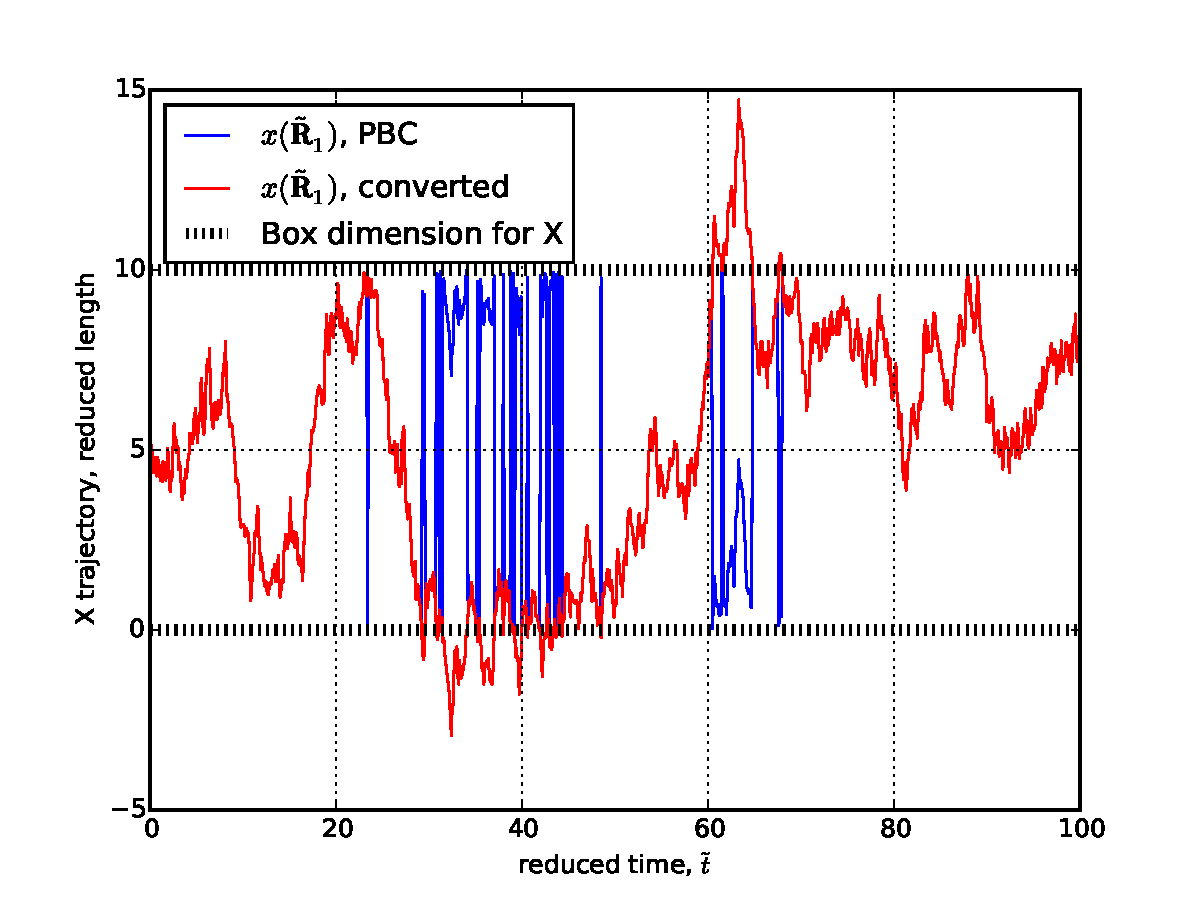
\includegraphics[width=\textwidth]{figures/converting_trajectory.pdf}
    \caption{Test results for trajectory conversion. Blue color represent the trajectory using periodic boundary condition (PBC) and the red color represent the converted data. The test is done using pure Brownian motion with 100 reduced time step, and trajectory is involved only for x-coordinate of the first beads among 100 beads on the system.}
    \label{fig:traj_conv}
  \end{figure}

  \section{Pair Correlation Distribution}
  The pair correlation distribution, $\rho(\mathbf{r}_1, \mathbf{r}_2$, is one of the important distribution function to show the structure information. There are various relation exist with spatial or reciprocal information.
  \subsection{Basic Definition started with Canonical Ensemble}
  For given canonical ensemble $(N, V, T)$, let $Z$ be configurational integra, partition function:
  \begin{equation}
    Z = \int d\mathbf{r}_1,\cdots d\mathbf{r}_N \exp\left(-\beta U\right),
  \end{equation}
  where $\beta$ be Boltzmann factor. Then, the probability of an elementary configuration is expressed by
  \begin{equation}
    P(\mathbf{r}_1, \cdots, \mathbf{r}_N)d\mathbf{r}_1\cdots d\mathbf{r}_N = \frac{\exp\left(-\beta U\right)}{Z}d\mathbf{r}_1\cdots d\mathbf{r}_N.
  \end{equation}
  Consider the case for reduced probability:
  \begin{equation}
    P^{(n)}(\mathbf{r}_1,\cdots,\mathbf{r}_n)=\frac{1}{Z}\int\exp\left(-\beta U\right)d\mathbf{r}_{n+1}\cdots d\mathbf{r}_N,
  \end{equation}
  where $n<N$ and superscript $(n)$ for $P$ denote probability reduced by $N-n$.

  
\end{appendices}

\printbibliography



\end{document}

\message{ !name(brief_Brownian_dynamics.tex) !offset(-911) }
